

%\documentclass[journal,draftcls,onecolumn]{IEEEtran}
\documentclass[journal]{spie}
%\renewcommand{\baselinestretch}{1.65}
\usepackage[]{times}

\usepackage{subfig}
\usepackage{listings}

\usepackage[sort, numbers, super]{natbib}

\usepackage{hyperref}

\usepackage{soul}
%\usepackage[pdftex]{graphicx}
\usepackage[]{graphicx}
\usepackage{url}
   \usepackage{siunitx}

%\newcommand {\EDIT} {\ul}		% show underlined edits.
%\newcommand {\EDIT} {}		    % show underlined edits.

\usepackage{multicol}
\usepackage{amsmath}
\usepackage{overpic}

\usepackage{xcolor}
\definecolor{Mauve}{rgb}{0.6,0.3,0.6}  % added Feb 2013

\pagestyle{plain}    
\begin{document}


\title{Schematic Driven Silicon Photonics Design \\
(Invited)}

\author{Lukas Chrostowski\supit{a}, 
Zeqin Lu\supit{a}, 
Jonas Flueckiger\supit{a},
James Pond\supit{b}, 
Jackson Klein\supit{b},
Xu Wang\supit{b},
Sarah Li\supit{a}, 
Wei Tai \supit{a}, 
En Yao Hsu\supit{a}, 
Chan Kim\supit{a}, 
John Ferguson\supit{c},
Chris Cone\supit{c}
\skiplinehalf
\supit{a}Department of Electrical and Computer Engineering, \\
University of British Columbia, Vancouver, British~Columbia, Canada \\
\supit{b}Lumerical Solutions Inc.,  Vancouver, British~Columbia, Canada \\
\supit{c}Mentor Graphics Corporation, Portland, Oregon, USA
}

\maketitle


%\lstset{language=Python,
%  basicstyle=\scriptsize, 
%  frame=single,tabsize=2, captionpos=b,breaklines=true,showstringspaces=false,
%  morecomment=[l]{\#},morestring=[b][\color{blue}]",morestring=[b][\color{blue}]'
%}
%\lstset{frame=shadowbox, xleftmargin=3mm, framexleftmargin=2mm, rulesepcolor=\color{blue}}
%\lstset{columns=flexible}

%\lstset{language=C,
%  basicstyle=\scriptsize, 
%  frame=single,tabsize=2, captionpos=b,breaklines=true,showstringspaces=false,
%%  morecomment=[l]{\#},morestring=[b][\color{blue}]",morestring=[b][\color{blue}]'
%}
%\lstset{frame=shadowbox, xleftmargin=3mm, framexleftmargin=2mm, rulesepcolor=\color{blue}}
%\lstset{columns=flexible}
%
%\lstset{language=bash,
%  basicstyle=\scriptsize, 
%  frame=single,tabsize=2, captionpos=b,breaklines=true,showstringspaces=false,  morecomment=[l]{*},   commentstyle=\color{DarkGreen}
%}
%\lstset{frame=shadowbox, xleftmargin=3mm, framexleftmargin=2mm, rulesepcolor=\color{blue}}
%\lstset{columns=flexible}
%
%
\lstset{language=Matlab,
frame=single,tabsize=2, captionpos=b,breaklines=true,showstringspaces=false,
%  aboveskip=3mm,
%  belowskip=3mm,
  columns=flexible,
  basicstyle={\tiny\ttfamily},
  numbers=none,
  numberstyle=\tiny\color{gray},
  keywordstyle=\color{blue},
  commentstyle=\color{DarkGreen},
  stringstyle=\color{Mauve},
  breakatwhitespace=true
}
\lstset{frame=shadowbox, xleftmargin=3mm, framexleftmargin=2mm, rulesepcolor=\color{blue}}
\lstset{columns=flexible}
%\lstset{basicstyle=\tiny}  % perhaps too small
%\lstset{basicstyle=\scriptsize\ttfamily}  % perhaps too big?
%\lstset{basicstyle=\tiny\ttfamily}  % perhaps too big?





\begin{abstract}

Electronic circuit designers commonly start their design process with a schematic, namely an abstract representation of the physical circuit.  In integrated photonics on the other hand, it is very common for the design to begin at the physical component level.  In order to build large integrated photonic systems, it is crucial to design using a schematic-driven approach.  This includes simulations based on schematics, schematic-driven layout, layout versus schematic verification, and post-layout simulations.   This paper  describes such a design framework implemented using Mentor Graphics and Lumerical Solutions design tools.  In addition, we describe challenges in silicon photonics related to manufacturing, and how these can be taken into account in simulations and how these impact circuit performance.


%This paper describes design methodologies developed for silicon photonics integrated circuits.  The approach presented is inspired by methods employed in the Electronics Design Automation (EDA) community.  This is complemented by well established photonic component design tools, compact model synthesis, and optical circuit modelling.   A generic silicon photonics design kit, as described here, is available for download at \url{http://www.siepic.ubc.ca/GSiP}.

\end{abstract}

\keywords{silicon photonics design, photonic integrated circuits design, electronic design automation (EDA), manufacturing variability, corner analysis, Monte Carlo simulation}


\section{Introduction}\label{sec1}

In electronic circuit design, the complexity and scale of designs necessitated multi-user collaboration.  Namely, a team of designers with different roles, such as concept and system architect, simulation expert, and layout designer, is required to implement a chip design.  In addition, there is another team, associated with the foundry that fabricates the designs, that includes device designers and process design kit developers.  The typical electronic design process begins with a schematic, namely an abstract representation of the circuit.  This requires that the foundry provides device models and layouts, embedded in a ``Process Design Kit'' (PDK) that can be used by circuit designers for their circuit simulations and to create their layout.  This partitioning of tasks is illustrated in Figure~\ref{Process_Design}.

\begin{figure}[tbp]
	\centering
	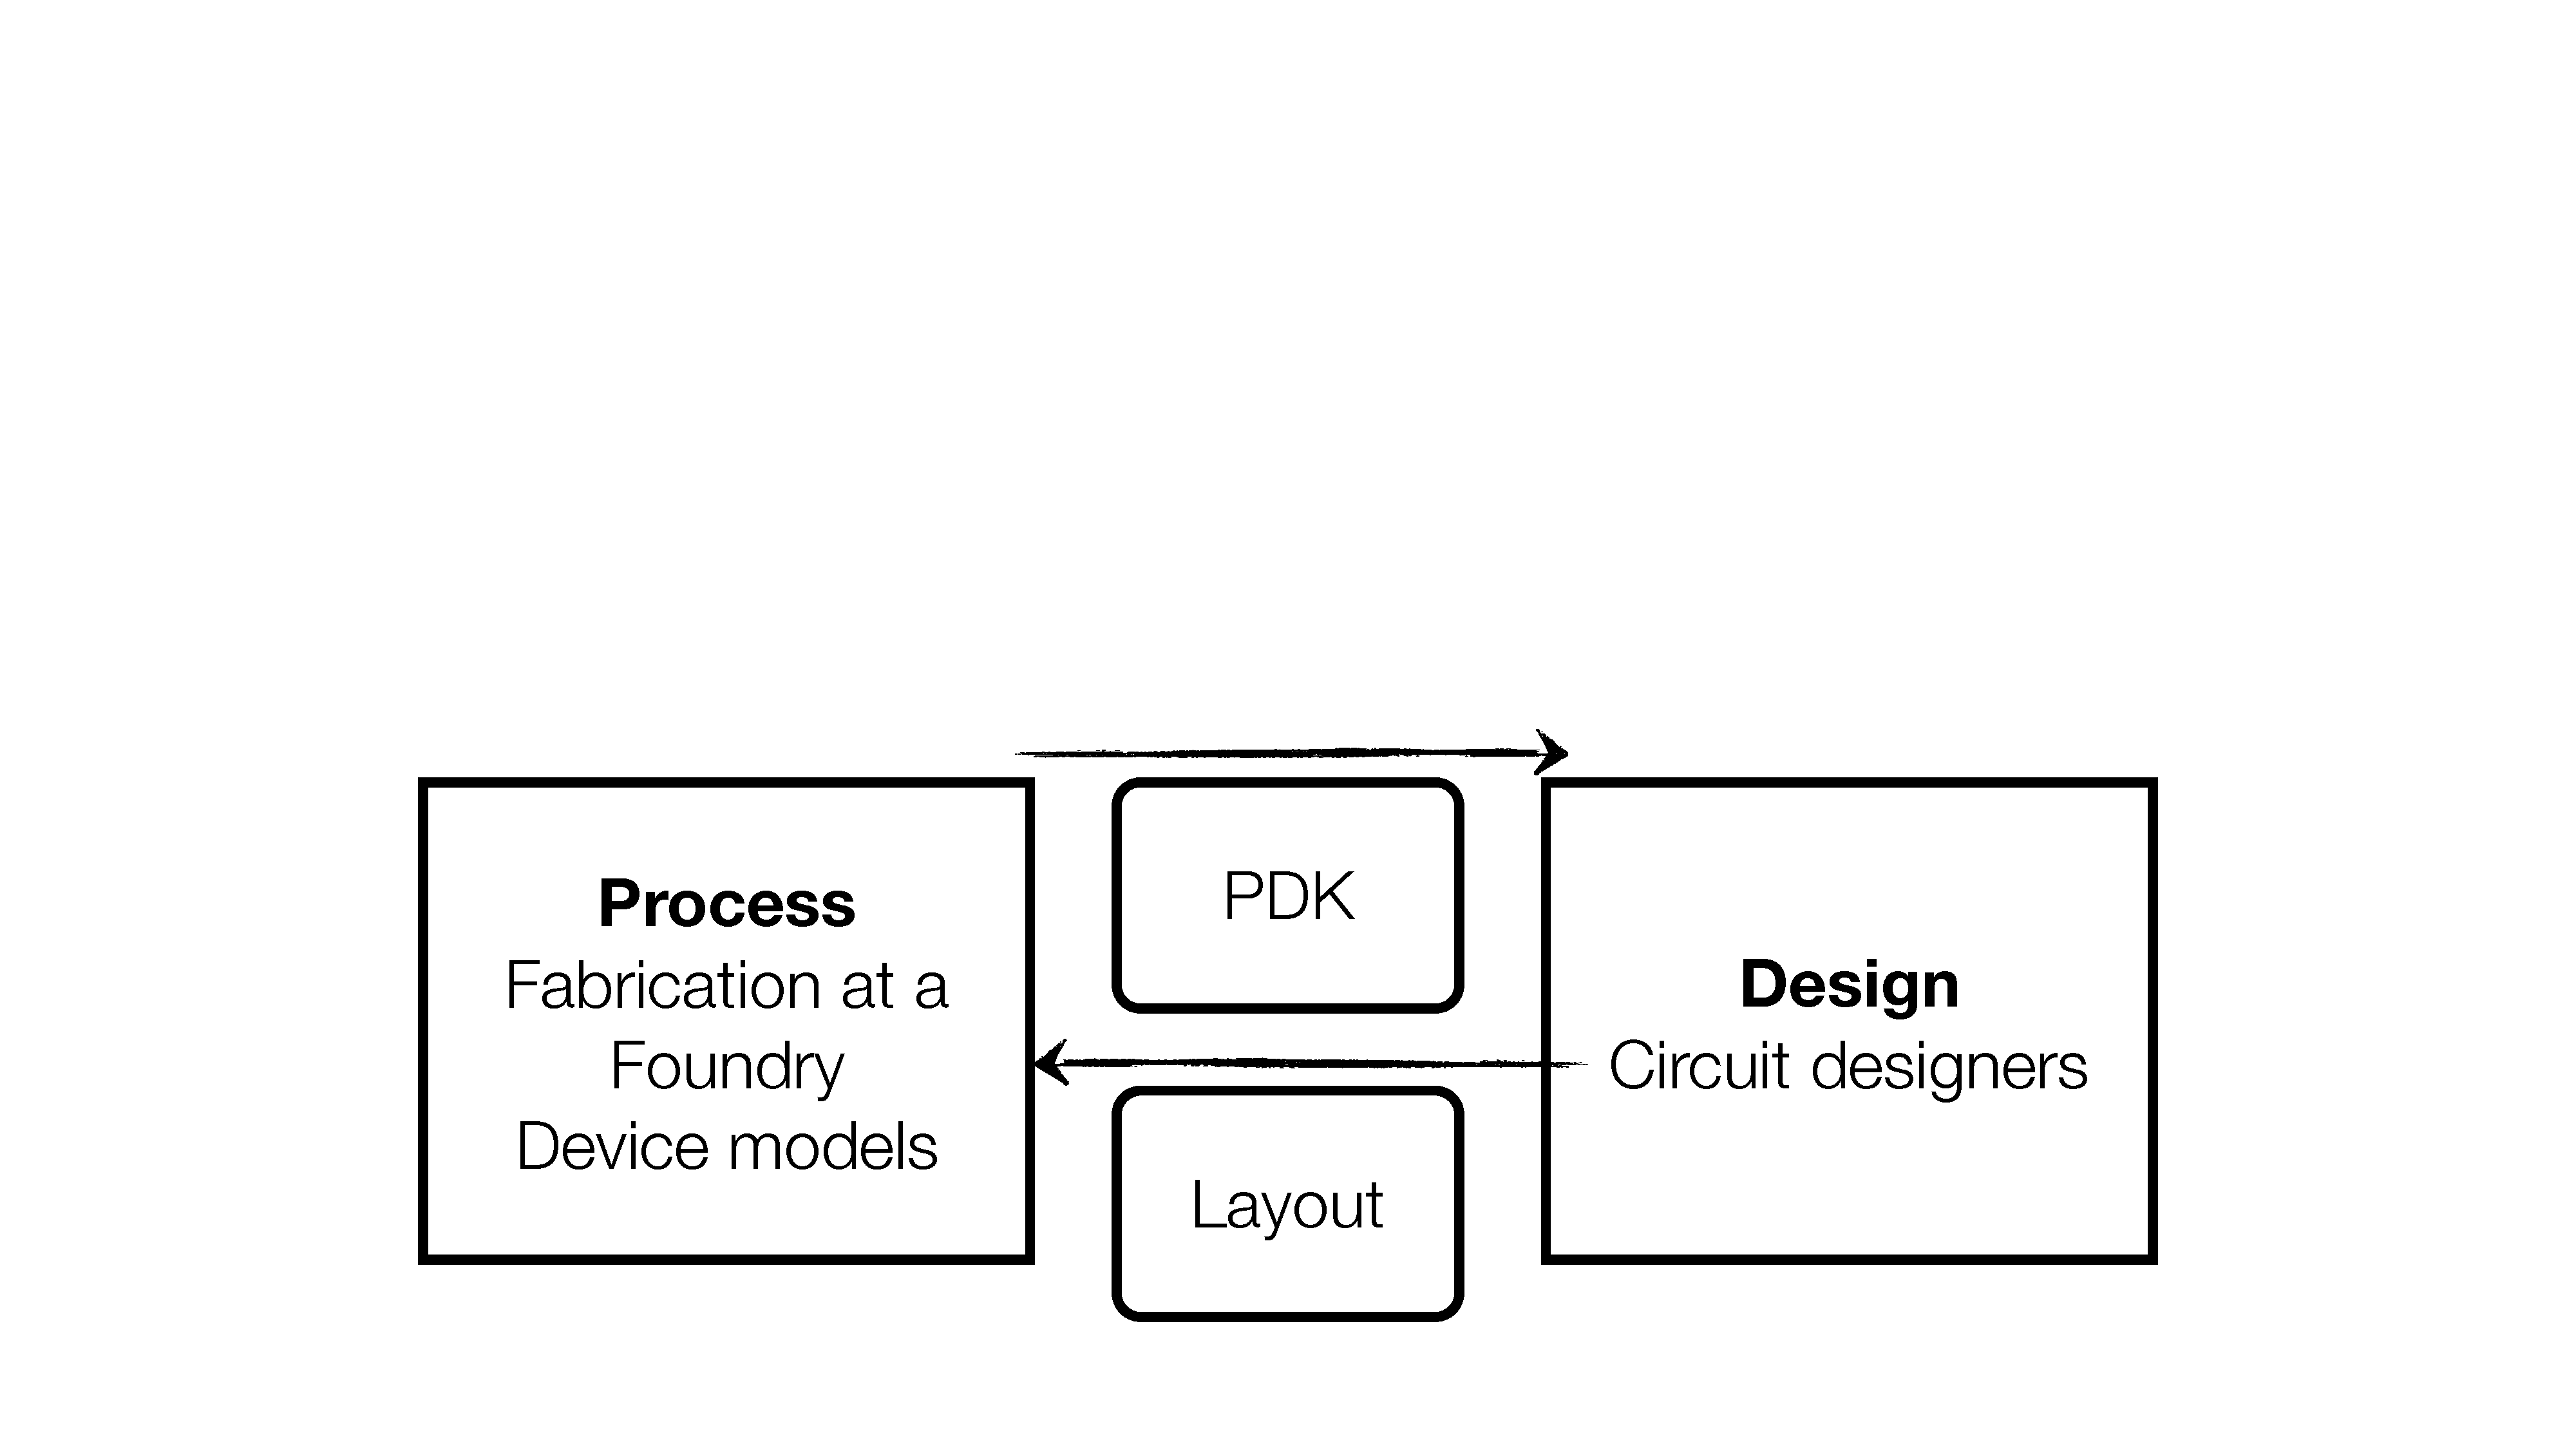
\includegraphics[width=0.5\textwidth]{../figs_paper/Process_Design.pdf}
    \caption[]{The partitioning of tasks between the foundry and the circuit designer.}
    \label{Process_Design}
\end{figure}



In integrated photonics design on the other hand, it is often one person who is responsible for all stages of the design.  Furthermore, the design process is usually ``bottom-up'', where the design begins with the physical components, and gradually builds up into a system.   In order to build large integrated photonic systems, it is crucial to 1) have a design methodology that allows for teams of designers with various roles to collaborate, and 2) have a capability that includes abstract representations (e.g., schematics) with a link to the physical implementation (layout).  

The proposed methodology is based on the electronic IC ecosystem.  This includes simulations based on schematics, schematic-driven layout, layout versus schematic verification, and post-layout simulations.   We have implemented a design framework using Mentor Graphics and Lumerical Solutions design tools that implements the above requirements, as described References \citen{chrostowski2014design} and \citen{chrostowski2015silicon}.

This paper expands upon the design methodology described previously by adding:
\begin{enumerate} 
\item Post-layout simulations
\item A choice in design style -- Schematic-Driven Design versus Layout-Driven Design
\item Manufacturing variability simulations (Monte Carlo)
\end{enumerate}
In particular, this paper emphasizes the importance of post-layout simulations.  We describe challenges in silicon photonics related to manufacturing, how manufacturing variability can be taken into account in post-layout simulations, and how these simulations can predict the impact of variability on circuit performance.

\section{Schematic-Driven Design}


First, we review the schematic-driven design approach described in References \citen{chrostowski2014design} and \citen{chrostowski2015silicon}, and illustrated in Figure~\ref{SDDvsLDD}.   This design flow is aimed at highly-complex silicon photonic circuits, analogous to how they are designed in the electronics industry.  Here, the design flow starts with an abstract representation, i.e., a circuit schematic.  We begin with symbols for the components,  place them on a schematic, and connect them.   This allows us to immediately simulate the circuit by providing the desired stimulus.  Behind the scenes, there are component models.  The designer does not need to develop them, since they are provided in the design kit.  Advanced PDKs will include active optical components, and electronics.  

\begin{figure}[tbp]
	\centering
	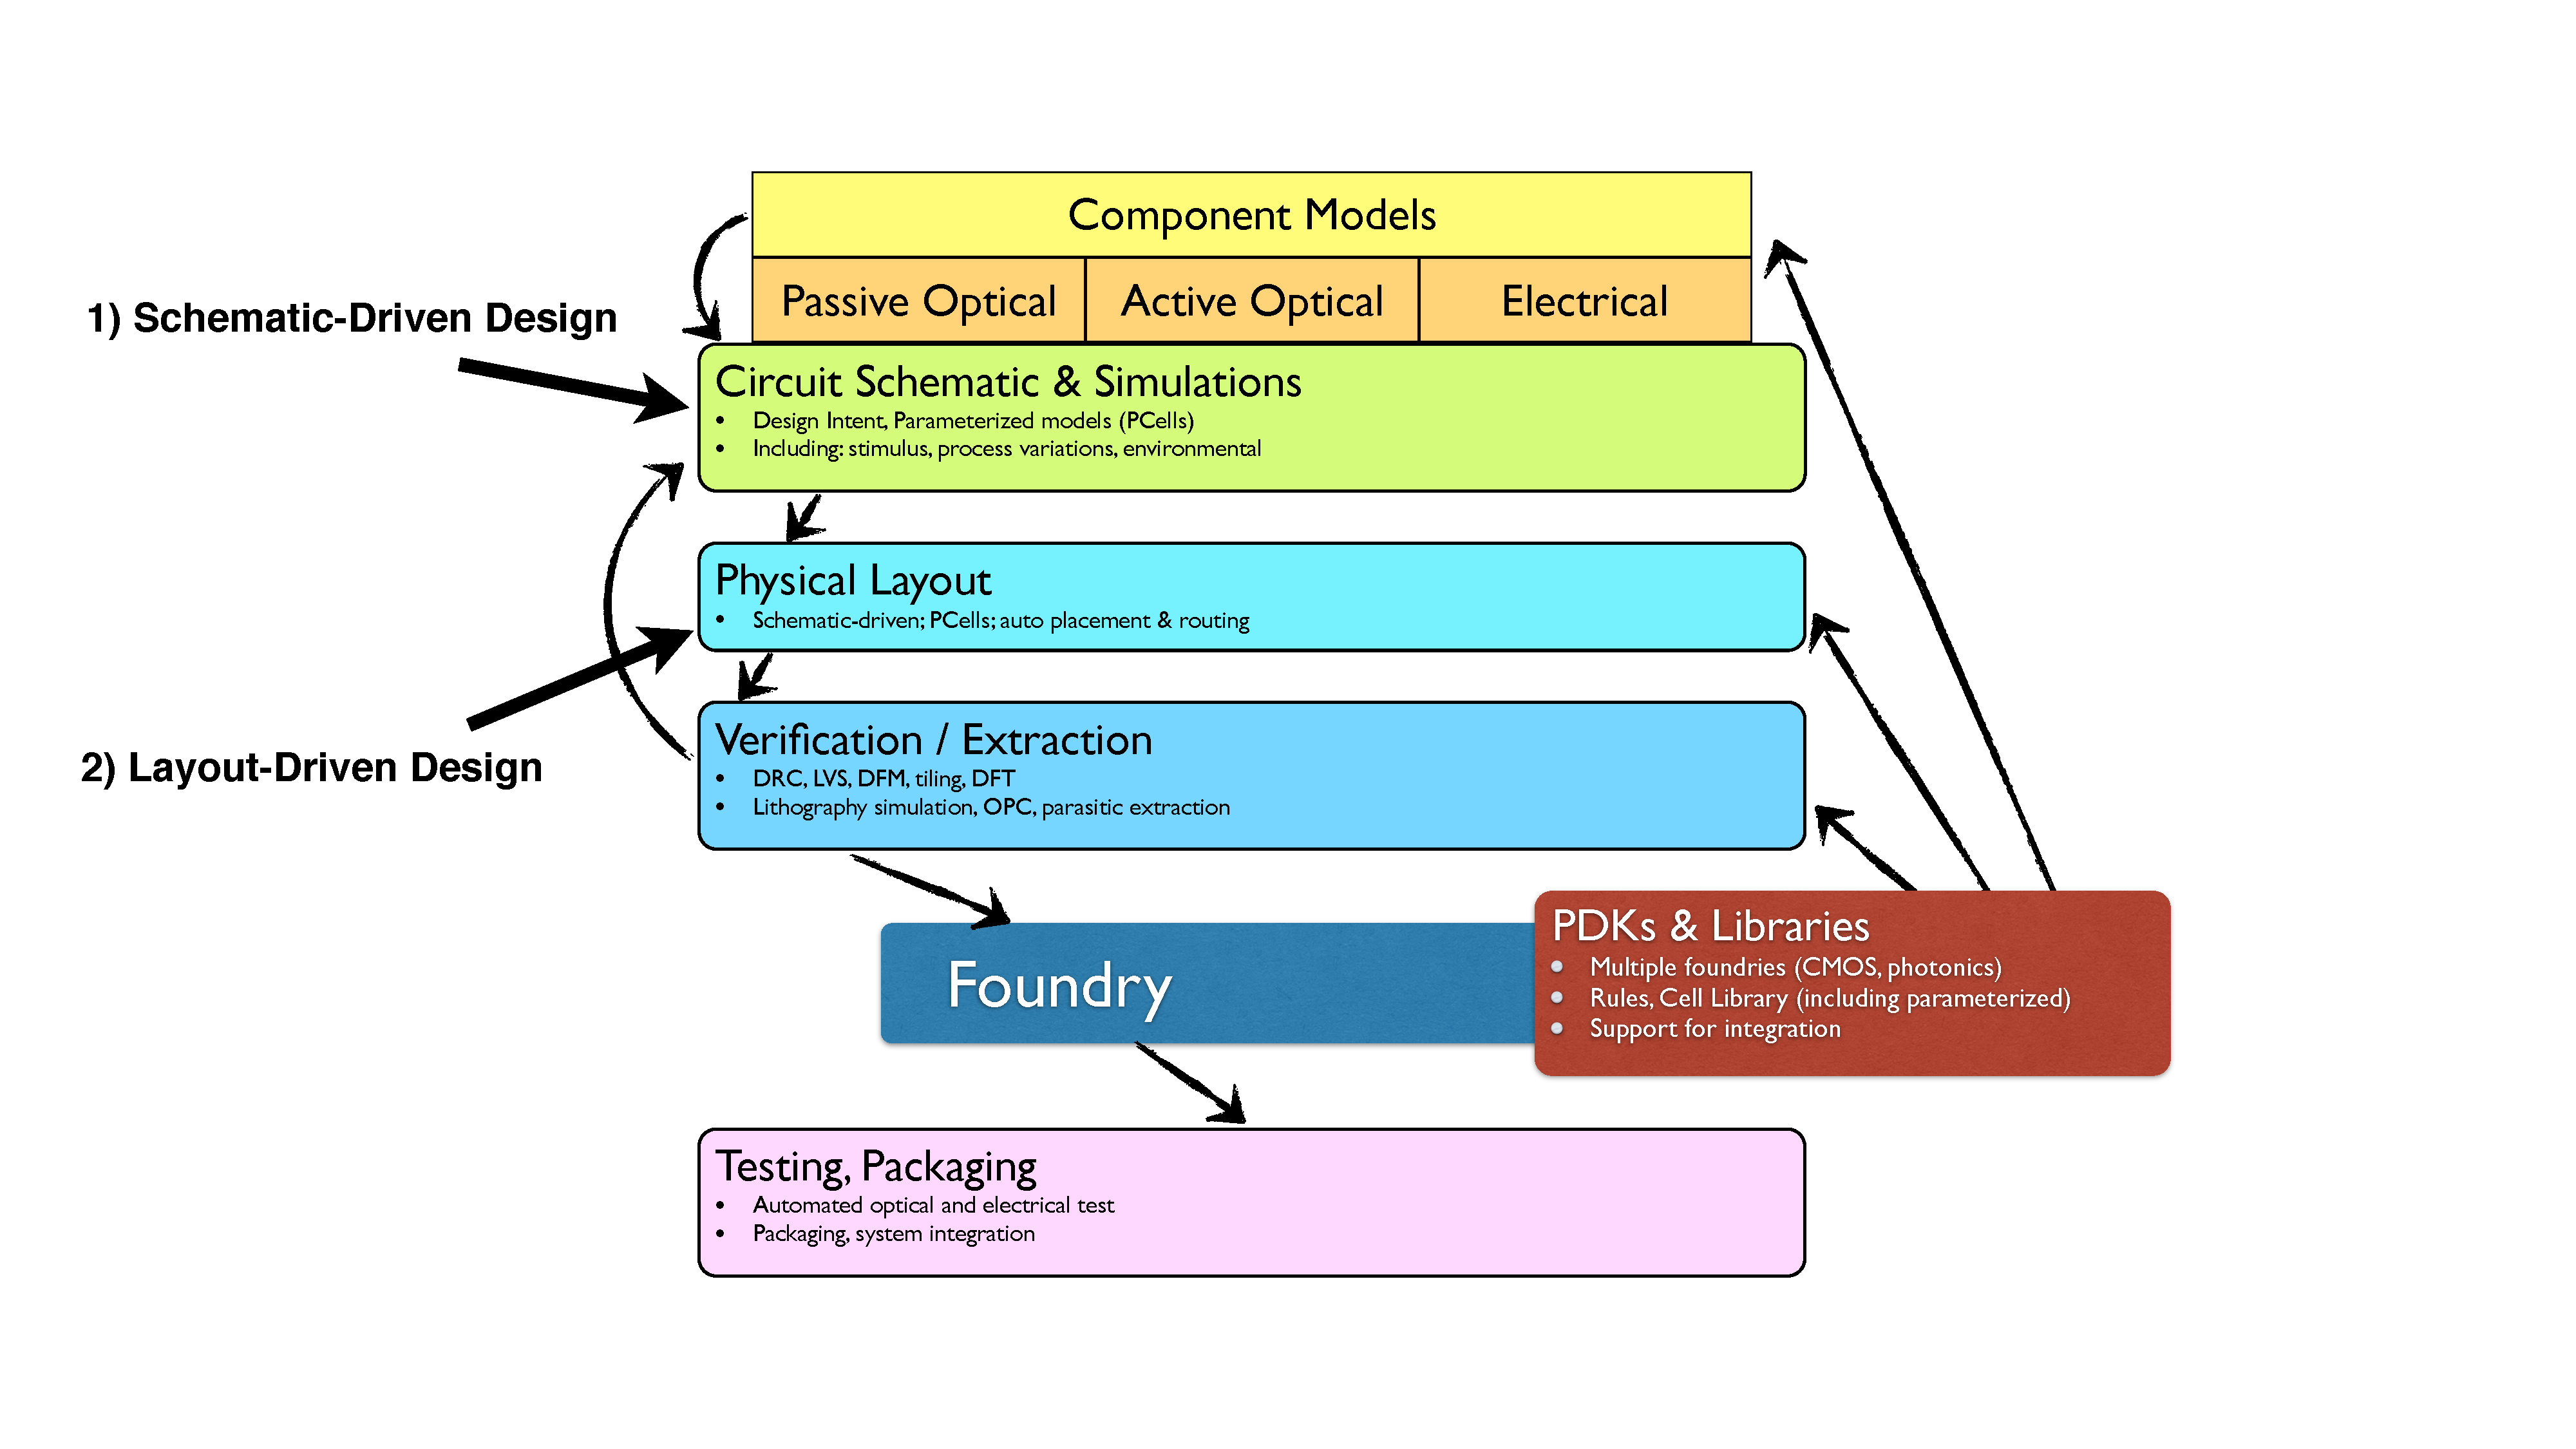
\includegraphics[width=0.9\textwidth]{../figs_paper/SDDvsLDD.pdf}
    \caption[]{Design methodology based either on 1) Schematic-Driven Design, or 2) Layout-Driven Design.}
    \label{SDDvsLDD}
\end{figure}


In this flow, the layout is created on the basis of the schematic, as shown in Figure~\ref{SDL_pic_2}.  The software aids the designer in creating the layout by reading the schematic as the layout is generated; specifically, component placement can be inferred from the schematic, and the connectivity between components is maintained to aid in the routing.

\begin{figure}[tbp]
	\centering
	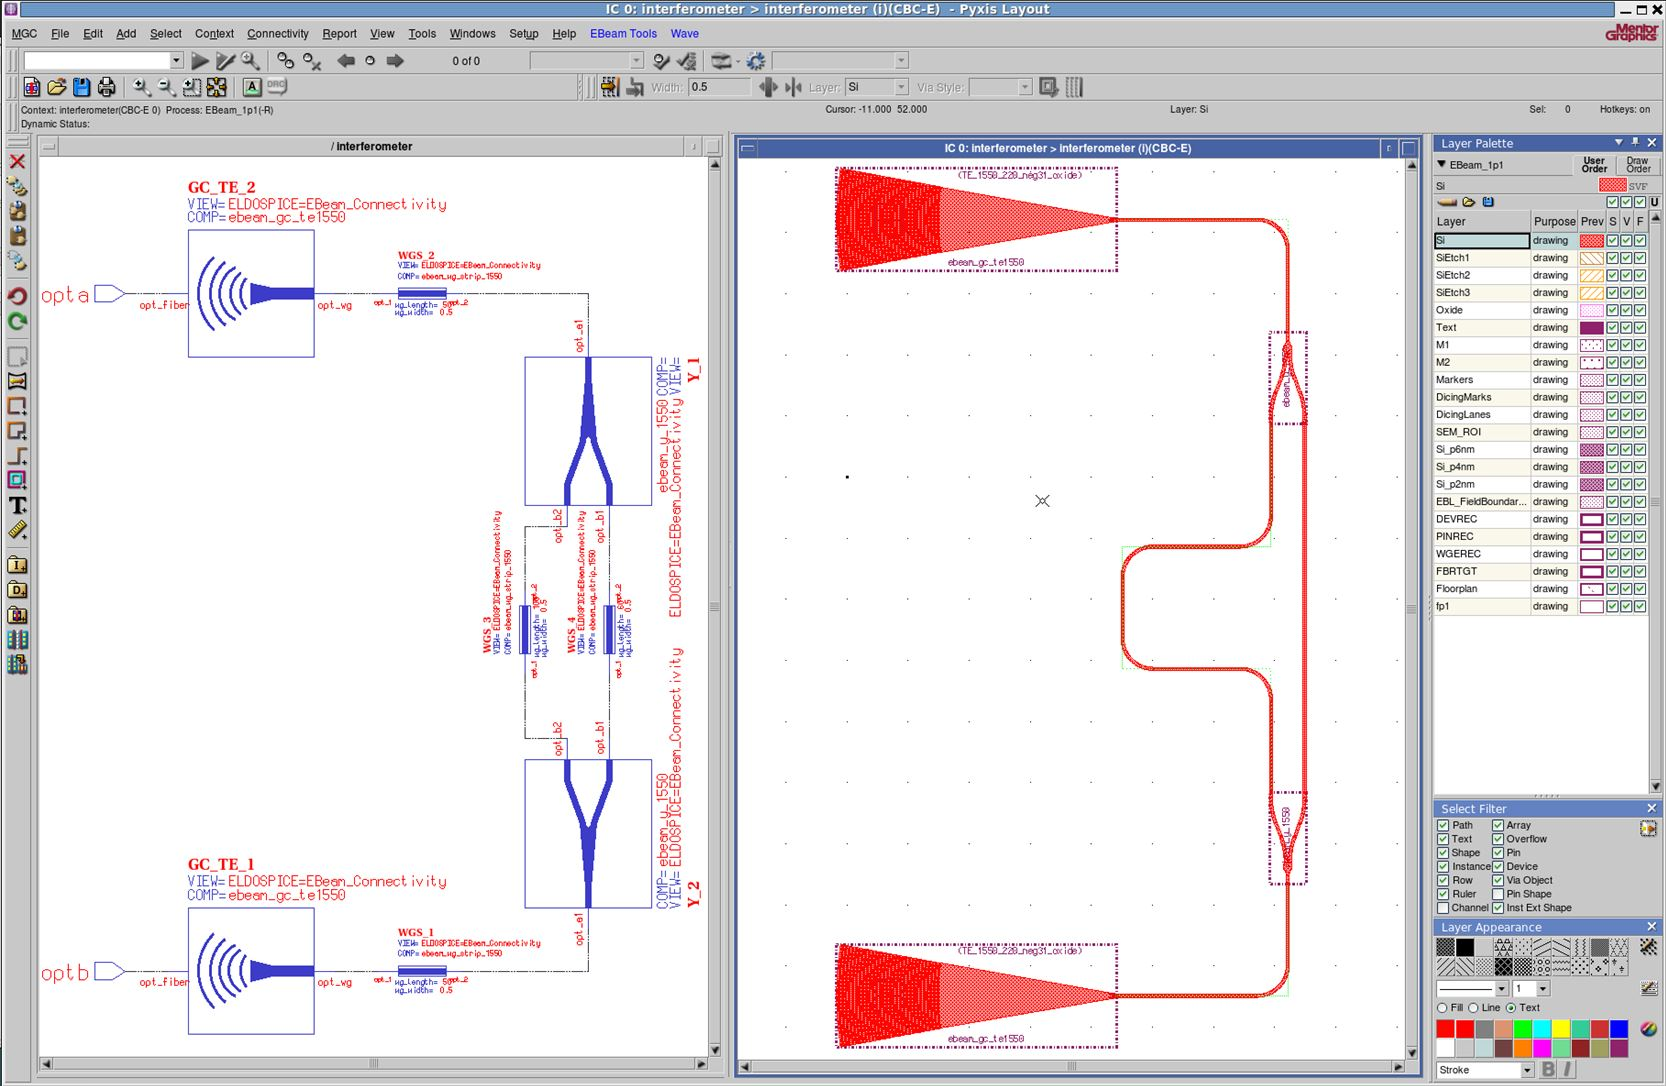
\includegraphics[width=\textwidth]{../figs_paper/SDL_pic_2.JPG}
    \caption[]{Schematic-Driven Design -- schematic capture (left), and schematic-driven layout (right).}
    \label{SDL_pic_2}
\end{figure}

The verification step involves two parts: 1) manufacturing verification (minimum features size, etc), known as Design Rule Check (DRC), and 2) functional verification, known as Layout Versus Schematic  (LVS).  The latter is critical for large circuits.  Since we have a schematic and a layout, we have the opportunity to compare them.  The LVS tool uses a set of rules to recognize the components and their connectivity in the layout, known as netlist extraction, and then compares the components and connectivity with the original schematic.  This verification step can identify incorrect connectivity, such as disconnected wires and waveguides, and component errors such as incorrect components or incorrect parameters.

Once the layout of the circuit is deemed to be correct, the LVS tool can extract the parameters from the layout and update the schematic.  For photonics, the lengths of your waveguides, as drawn, is often critical in determining performance.  For example, the lengths of the waveguides in an interferometer need to be calculated so that we can obtain an accurate estimation and simulation of the free spectral range (FSR). After the schematic is updated, the designer can re-simulate the circuit to verify that it operates as expected once the details (such as waveguide length in photonics, or parasitics in electronics) are included.


In contrast to the traditional photonics design approach, this design flow has a much more well established design kit, and enables rapid design of complex circuits, without having to spend time on modelling individual components.  This type of design has been critical to the success of the electronics industry where circuits have thousands to billions of components.

An evolution that is expected for integrated photonics design is that we are moving towards a methodology similar to CMOS design leading to a distinct skill sets.  For example, circuit designers will need to know the minimum of information about how a directional coupler works, but will not need to design them (the main knowledge required is that its function is similar to a beam splitter).  However, the circuit designer will be highly attuned to the performance criteria of the splitter (e.g., wavelength dependance of the splitting ratio, insertion loss, power splitting balance, sensitivity to manufacturing variations) and how these impact the circuit performance (e.g., extinction ratio, crosstalk).  This enables the circuit designer to focus on design at a higher level, including system implementation.


As the field of integrated photonics progresses, we expect that the industry will further evolve towards how CMOS electronics design is done.  In particular, this will lead to a partitioning of design tasks, with each task requiring a distinct skill set.
%An evolution that is expected for integrated photonics design is that we are moving towards a methodology similar to CMOS design leading to a distinct skill sets.  
For example, circuit designers will need to know the minimum of information about how a directional coupler works, but will not need to design them (the main knowledge required is that its function is similar to a beam splitter).  However, the circuit designer will be highly attuned to the performance criteria of the splitter (e.g., wavelength dependance of the splitting ratio, insertion loss, power splitting balance, sensitivity to manufacturing variations) and how these impact the circuit performance (e.g., extinction ratio, crosstalk).  This enables the circuit designer to focus on design at a higher level, including system implementation.


\subsection{Post-Layout Simulation}

Post-layout simulation refers to circuit simulations that are performed after the layout is created.  In the schematic-driven design flow, this involves extracting parameters from the layout, and updating the schematic.  However, there is another use case for post-layout simulations.  Namely, we desire the capability to simulate directly from a layout without requiring a schematic (e.g., for layouts created by a different designer,  layouts created using different software, and in general if the schematic is not available).

In this case, the LVS tool can be used to create a netlist representation of the circuit.  This is in fact easier to perform than the layout versus schematic operation described above, as it only requires the netlist extraction step.  The requirement for this functionality is that each component is supported by the library / PDK.  This is necessary so that the LVS tool can recognize the devices correctly, and label them with the appropriate component model.  We have added additional marking layers to the components, to aid the LVS identify the components, their names, where the input / output ports are, and their port names.

After the layout extraction is done, the circuit simulator tool is used as before to perform simulations, based on the netlist.

\section{Layout-Driven Design}

The capabilities developed for post-layout simulation allow us to consider another design methodology, namely layout-driven design.   This second approach begins with the layout, as shown in Figure~\ref{SDDvsLDD}.  First the designer creates a layout, then simulates it directly from the layout.  The simulation is performed in two steps: a) netlist extraction and b) circuit simulations.  

This approach may be appealing to traditional photonics designers who have independent design stages: device modelling, circuit design, and layout.  In this traditional flow, there is no communication between these stages, hence verification and post-layout simulation is challenging.  In the case of separate tools, the need for schematics may not even be obvious or required.  For these designers, the benefit of including post-layout simulations in the layout-driven design flow is that accurate simulations can be generated based on the design.  An inspection of the simulation results, and comparison with expectations, is an excellent verification step.

Another advantage of the layout-first approach is that it provides insight into what is physically realistic, prior to doing abstract circuit design in a schematic.  For example, creating a layout first gives the designer insight into how large the library components are, how long the waveguides will need to be, how far apart the components will need to be, how many waveguide crossings will be required, etc.  

Another design option is to create a draft layout with arbitrary component parameters and use the post-layout simulation functionality to create the files necessary for circuit modelling.  Once the simulation project is set up, including all components found in the layout, as well as a stimulus (e.g., laser) and analysis instruments (e.g., detectors), the designer can proceed to optimize the design within the circuit modelling tool.  For example, in a WDM ring modulator transceiver, the choice in ring resonator parameters can be performed in the circuit modelling tool, using the realistic simulation environment created from the layout extraction tool.  In such a design flow, it is also important to have the capability for the component parameters to be synchronized between the circuit simulation and the physical layout.

Clearly, there are several design flows that are enabled by the capability of extracting the netlist from the physical layout.  The layout-driven design approach is likely to be attractive for small circuit designs.

Both of these design flows (schematic-driven and layout-driven) require that there is a connection between the layout and the schematic, and in both directions.  Both need a library of components, containing component models, component layouts, and component layout recognition rules (called an LVS rule deck).  The biggest challenge for the designer is to obtain access to all the necessary pieces, namely to have access to a state-of-the art PDK similar to those available in the electronics industry.  





\section{Layout Extraction}

In this section, we provide further details on the layout extraction and netlist generation procedure.  
As discussed above, extracting the netlist from the layout is important for two reasons: 1) to verify the layout, with respect to the abstract (schematic) representation, 2) to simulate the as-drawn layout, which will include the precise waveguide lengths and component position information.  The post-layout simulation is an important verification step to ensure that no errors were introduced during the layout (e.g., disconnected waveguides leading to back-reflections).

In this section, we describe an example layout -- a Mach-Zehnder Interferometer circuit as shown in Figure~\ref{MZI_circuit2}.  It consists of two fibre grating couplers, two broad-band splitters \cite{lu2015broadband}, and numerous waveguides and waveguide bends.  The netlist is extracted from the layout, either using Mentor Graphics Calibre Layout Versus Schematic (LVS), or using the open-source KLayout \cite{www_klayout} tool with the SiEPIC-EBeam-PDK add-on \cite{siepic-ebeam-pdk}.  The extracted netlist is shown in Listing~\ref{MZI_circuit2.spi}.  Although this is a simple circuit, the listing is quite long and involves 18 components.  
Each component includes the following information:
\begin{itemize}
\item The nets to which each component pin is connected to (e.g., N\$2)
\item The library which contains the component's compact model to be used for simulations (e.g., ``Design kits/ebeam\_v1.2'')
\item The component position in the layout (lay\_x, lay\_y)
\item Optionally, a position for the component to be used in drawing the schematic (sch\_x, sch\_y)
\item Component parameters, for components that are parameterized.  For the waveguides, the parameters are the waveguide width and length.    For bends, the parameters are the radius and the waveguide width.
\end{itemize}

In the above circuit, the waveguide is broken up into straight sections and waveguide bends.  The advantage of separately listing these components is that it allows the circuit simulation to be as detailed as possible.  For example, the circuit simulation can include:
\begin{itemize}
\item An accurate model for the waveguide bend, including the insertion loss, the optical phase through the device, and the reflections from the mode-mismatch from the straight-to-bend region.
\item Position information for all these components can be used for thermal modelling and for Monte Carlo simulations, as described below.
\end{itemize}
Such an approach is particularly useful if the designer has a choice of waveguide bend radius, and the impact of the bends is not known a priori.  A simulation with that includes numerous waveguide bends with a too-small bend radius would predict the Fabry-Perot cavities introduced by the small reflections at all interfaces.  

However, in many cases, the bend has already been optimized, analyzed and chosen so that it has little impact on the circuit performance.  In that case, precise knowledge of the bend location is not necessary to include in the circuit model, nor is the bend itself.  An alternative representation of the above circuit is one where the waveguides and bends are merged into a single waveguide object.  This approach reduces the size of the netlist, and improves on the performance of the circuit simulations.  One modification is made to the waveguide object as follows:
\begin{itemize}
\item The waveguide length includes the straight sections, and the waveguide bends.  The length of the waveguide bends is taken as $L = \pi r/2$, where $r$ is the radius taken at the centre of the waveguide.
\item The waveguide has an additional parameter, namely a vector of points, e.g., points=``((-59050, 5000), (-45690, 5000), (-45690, -117300), (-59050, -117300))''  [units of nanometers].  These are used in the Monte Carlo analysis described below.
\end{itemize}



\begin{figure}[tbp]
	\centering
	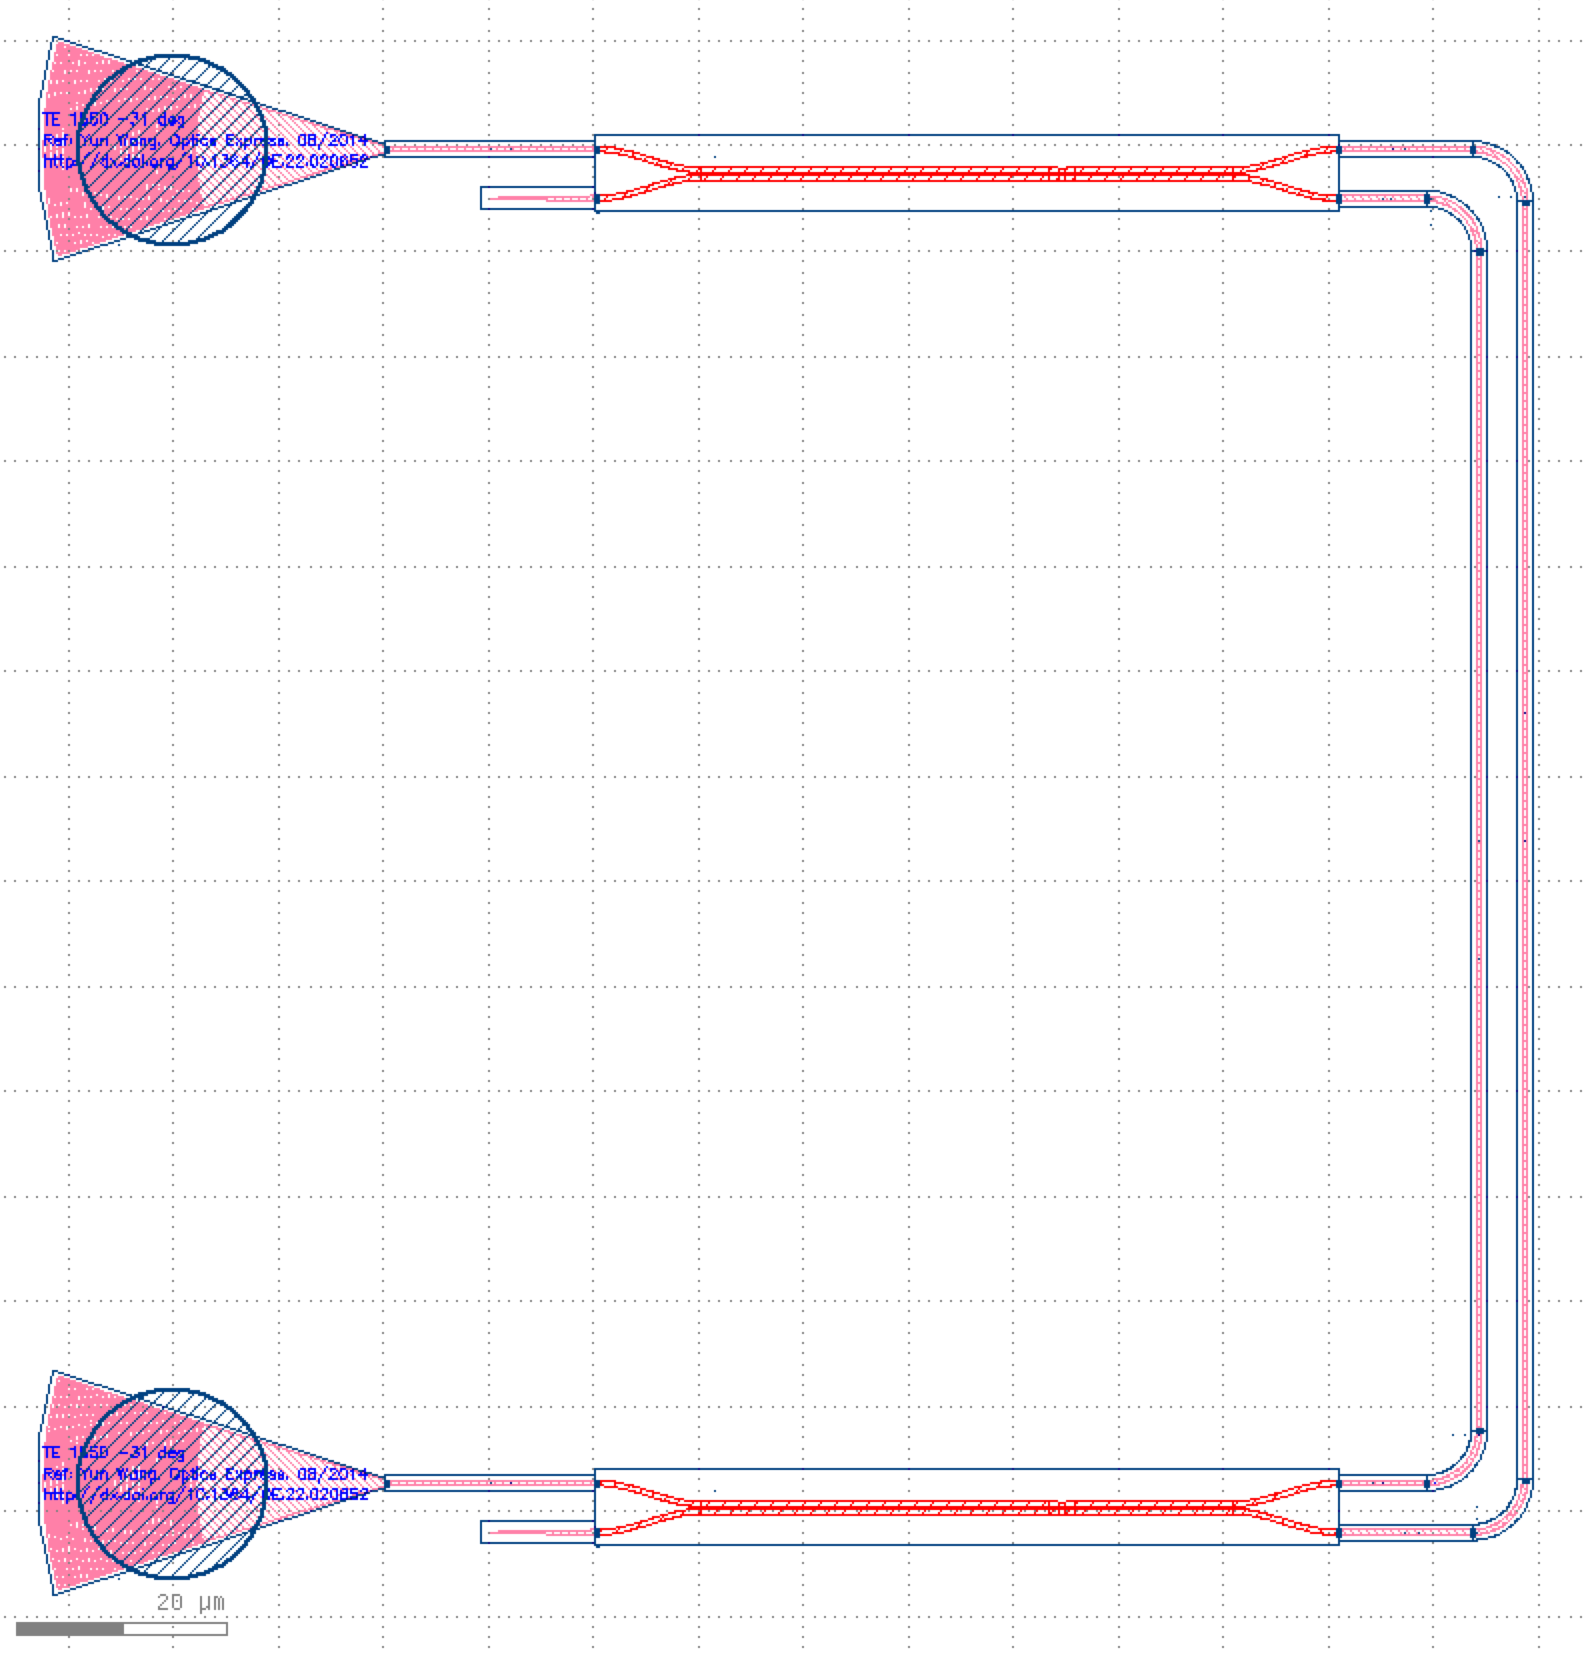
\includegraphics[width=0.5\textwidth]{../figs_paper/MZI_circuit2.png}
    \caption[]{Example layout of a Mach-Zehnder Interferometer circuit.}
    \label{MZI_circuit2}
\end{figure}

\lstinputlisting[language=Python, caption={Netlist, in SPICE format, for a Mach-Zehnder Interferometer circuit. This netlist includes all bends as separate components.},label=MZI_circuit2.spi]{MZI_circuit2.spi}

\lstinputlisting[language=Python, caption={Netlist, in SPICE format, for a Mach-Zehnder Interferometer circuit. This is a simplified netlist where the waveguides and bends are grouped into a single waveguide object.},label=MZI_circuit3.spi]{MZI_circuit3.spi}




\section{Circuit Simulations}
\label{sec:circuitsim}
We previously described how to perform circuit simulations of photonic circuits using compact models created from S-parameters which are simulated using 3D-FDTD or other numerical techniques\cite{chrostowski2014design, chrostowski2015silicon}.  This is a powerful technique since it allows any passive device to be represented, without having to establish expressions that describe the behaviour of the component.  Efficient circuit simulations can be by achieved by using S-parameters directly, in particular for frequency (wavelength) domain simulations, as the S-parameters are already wavelength dependant.  For time domain simulations, the circuit modelling tool internally converts the S-parameters into a time-domain representation.  

We provide an example of a Bragg grating cavity test structure layout in Figure~\ref{Bragg}, together with the simulations from the extracted netlist.  The response of the circuit deviates from the ideal Bragg grating cavity response, due to: 1) the grating coupler insertion loss, 2) the back-reflections from the grating couplers, and 3) the insertion loss and back-reflections from the tapers.  Ripples are observed in both the transmission and reflection spectra, that are not present in the ideal model.  Furthermore, the shapes,  positions, and oscillation frequencies of the ripples are dependant on the optical phases introduced by the various components, such as the waveguides.  Hence it is important to extract the lengths and device parameters for an accurate simulation.

\begin{figure}[tbp]
\begin{center}   
\subfloat[Layout of a Bragg grating cavity test structure.]{\label{Bragg1} 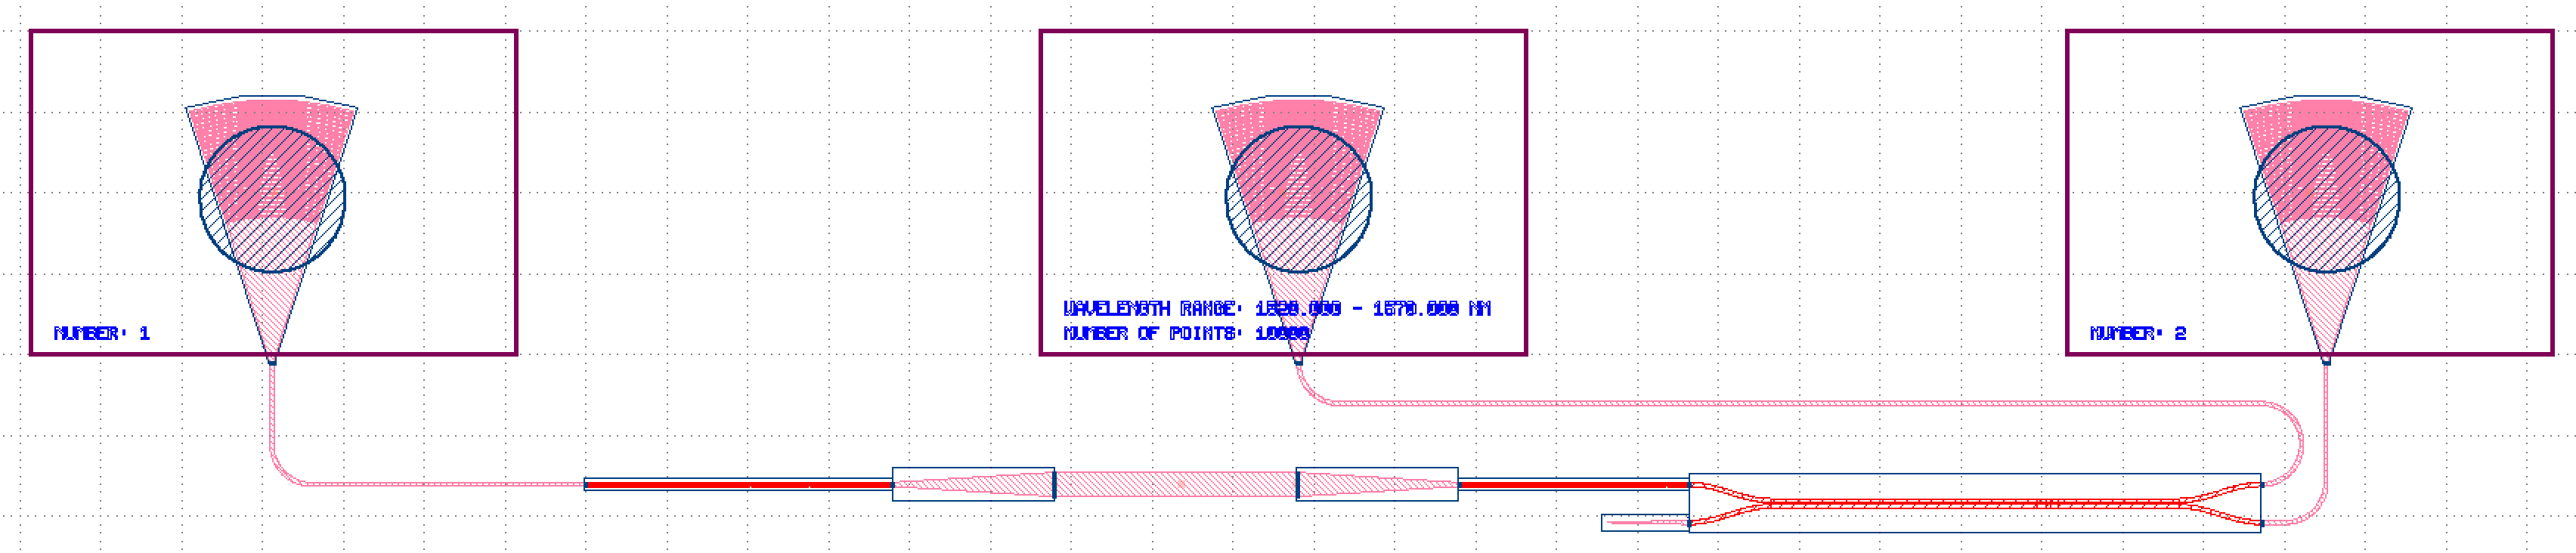
\includegraphics[width=0.8\linewidth]{../figs_paper/Bragg1} } \\
\subfloat[Zoom of the Bragg cavity, showing a portion of the Bragg grating and the taper.] {\label{Bragg2}
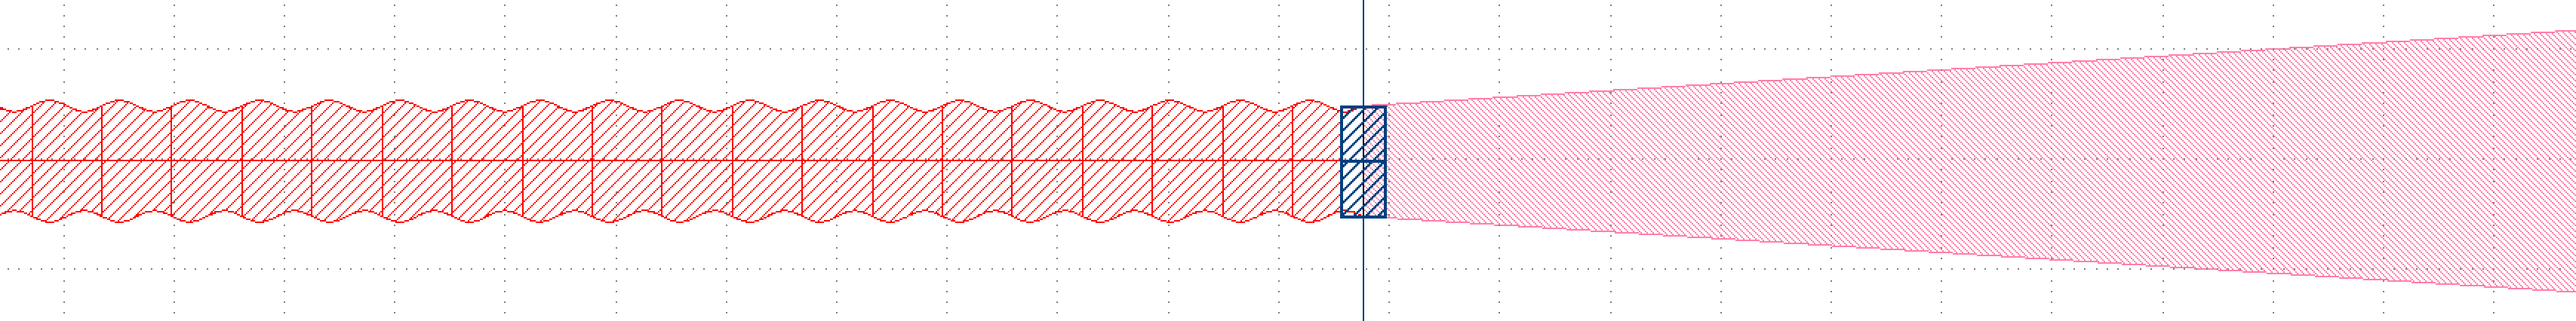
\includegraphics[width=0.8\linewidth]{../figs_paper/Bragg2} } \\
\subfloat[Circuit simulation of the Bragg grating test structure.] {\label{Bragg}
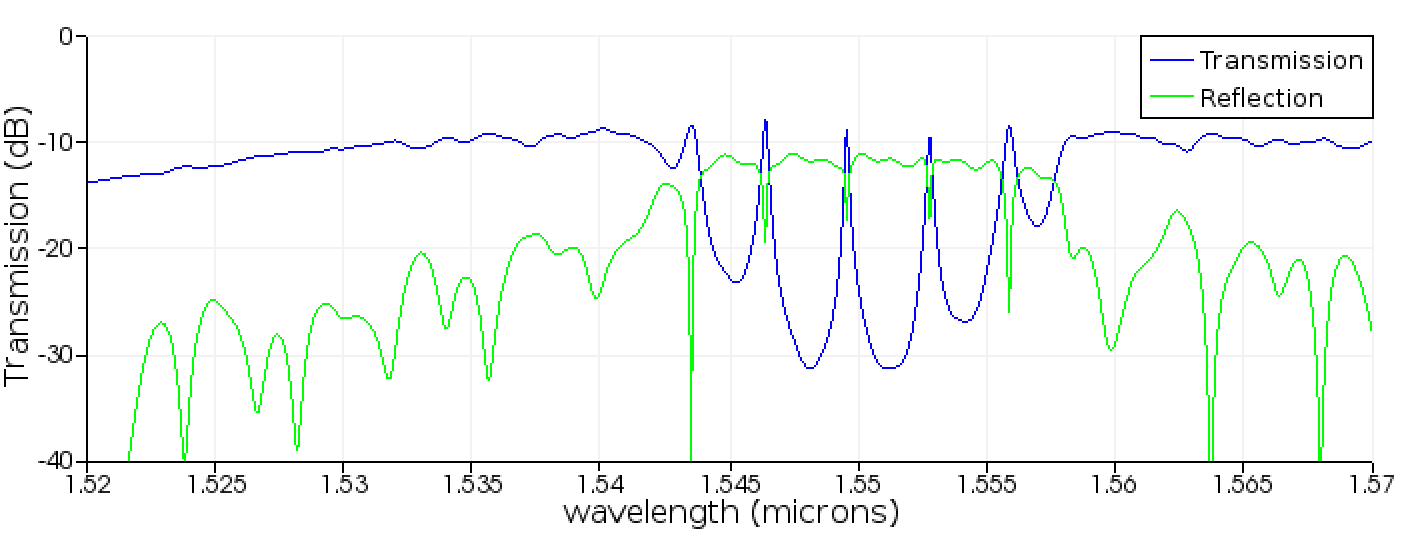
\includegraphics[width=0.8\linewidth]{../figs_paper/Bragg} }
\caption{Layout and simulations of a Bragg grating cavity.}
\label{Bragg}
\end{center}
\end{figure}



\graphicspath{{../figs_chris/}}

\begin{figure}[tbp]
	\centering
	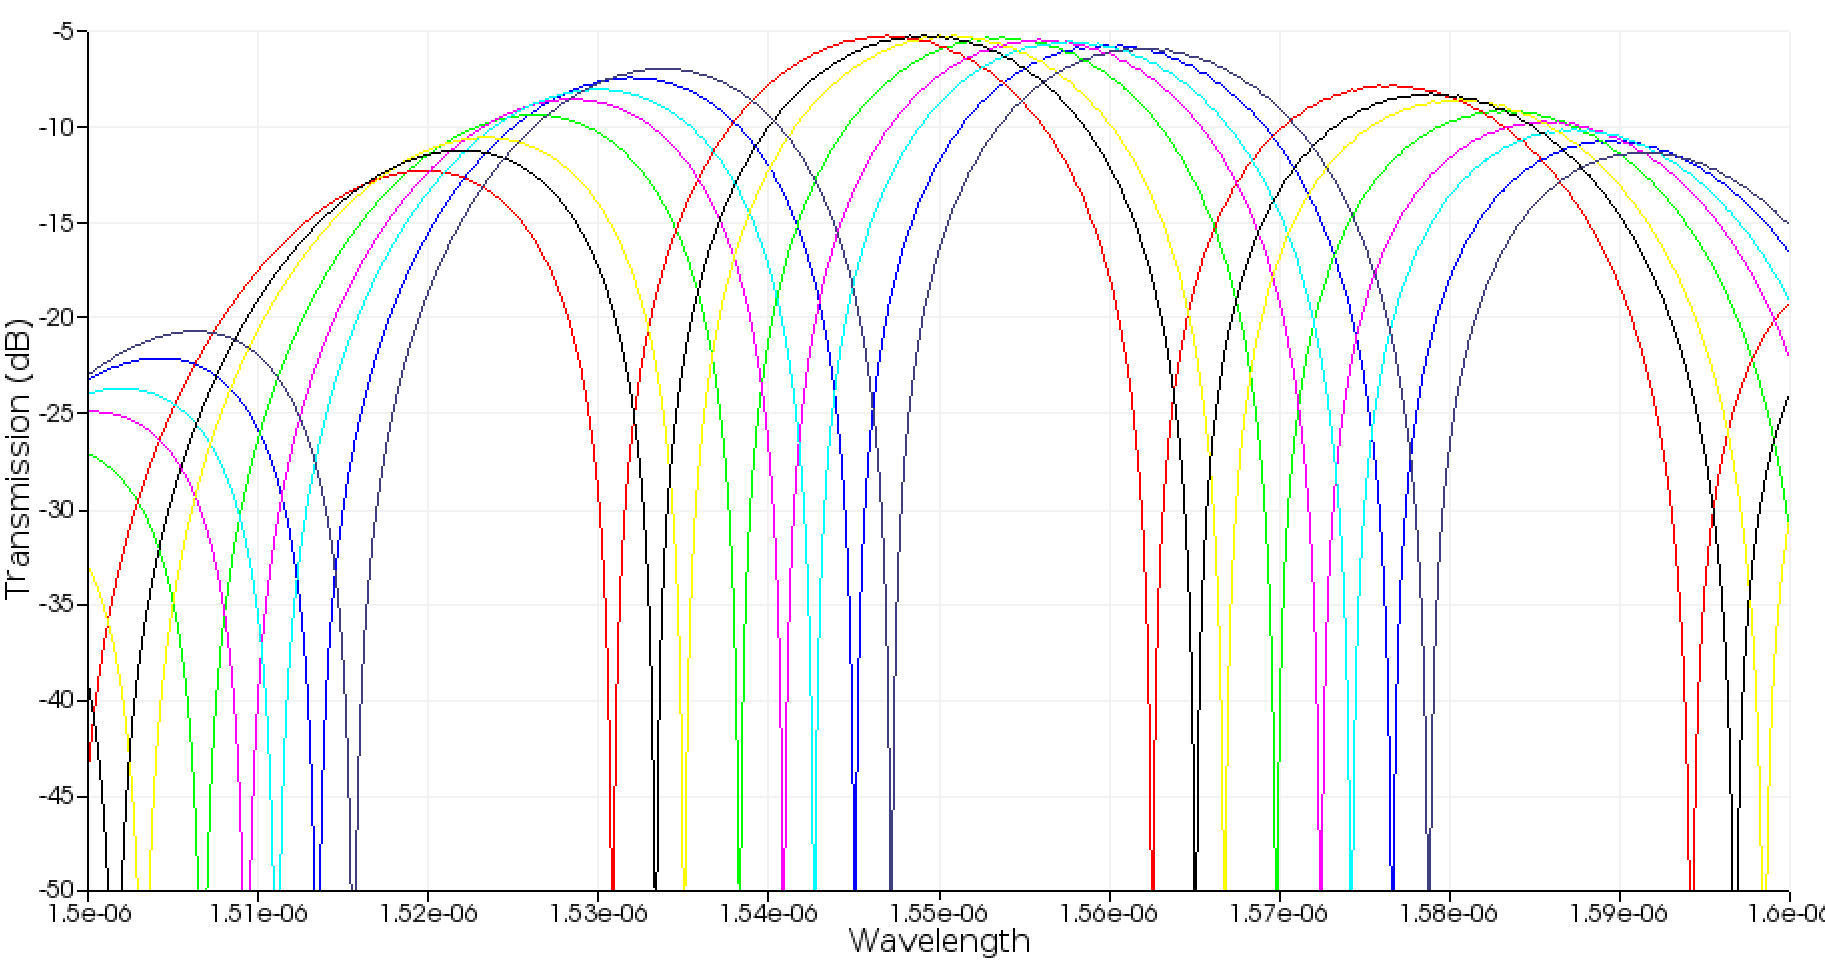
\includegraphics[width=0.8\textwidth]{../figs_paper/MZI_circuit2_MC.png}
    \caption[]{Monte Carlo simulation of the Mach-Zehnder Interferometer layout in Figure~\ref{MZI_circuit2}.}
    \label{MZI_circuit2_MC}
\end{figure}



%%%%%%%%%%%%%%%%%%%%%%%%%%%%%%%%%%%%%%%%%%%%%%%%%%%%%%%%%%%%%%%%%%%%%%
\section{Manufacturing Variability}
\label{sec:variability}
The high refractive index contrast of SOI permits sharp waveguide bends and ultra-small device sizes, making it promising for the development of densely integrated photonic circuits. However, silicon photonic devices face serious manufacturability challenges. Fabrication errors on either the waveguide width or waveguide thickness have a significant effect on the propagation constant of light, and, thus, circuits such as interferometers are highly sensitive to manufacturing, as shown in Figure~\ref{MZI_circuit2_MC}.

Thus, taking manufacturing variability into account in order to predict yield is critical for photonic integrated circuits. In the electronics community, corner analysis and Monte Carlo simulations are typically used to analyze fabrication variability; the former predicts the worst-case performance of the circuit, while the later creates histograms and distributions, and is based on statistical process variations.  In the simplest Monte Carlo approach, the same process variations are applied to all components in the circuit, thus the simulation considers common-mode variability only (e.g., all devices are slightly thicker).  

\subsection{Component models taking into account variability}
In order to perform Monte Carlo simulations, we require parameterized component models that are continuous with the variables of interest (e.g., thickness, width).  Although one approach is to simulate each component on a fine mesh (e.g., 0.1 nm steps in each deviation variable), this is computationally prohibitive.  We developed more efficient approaches, as follows.

\subsubsection{S-Parameter component models}
\label{SparamModel}
We begin by generating S-parameters for the corner cases (e.g., components with variations ($\Delta$w (nm), $\Delta$h (nm)) of (+20, +10), (+20, -10), (-20, +10) and (-20, -10)), as shown in Fig.~\ref{s-interpolation}(a).  For each Monte Carlo iteration, we interpolate the S-parameters for the desired thickness and width variation.  We implement this interpolation as a script within the component in Lumerical INTERCONNECT.  The inputs to the component are the thickness and width.
The model can also include multiple modes (e.g., TE and TM polarization).

We use a multidimensional spline interpolation method, which allows for the estimation of the amplitude and phase for each S-parameter taking into account its dependency on multiple parameters, such as the optical wavelength (or frequency), thickness and width.  S-parameters passivity and reciprocity can also be tested and enforced, to avoid violating energy conservation laws.  

This approach can be applied to components such as directional couplers, where the phase through the device is dependant on the thickness and width of the waveguide.  Two directional couplers can be connected to create a ring resonator sub-circuit, and the performance of the ring resonator (resonance frequency, free spectral range, extinction ratio) will vary with the thickness and width variability introduced into the directional coupler model.  As an example, Fig.~\ref{s-interpolation}(b) shows the S-parameters for the four process corners, and one example interpolated case for a 2$\times$2 splitter, a device described in Ref.~\citen{lu2015broadband}. 


\begin{figure}[tbp]
	\centering
\subfloat[] {\label{S_Interpolation1}
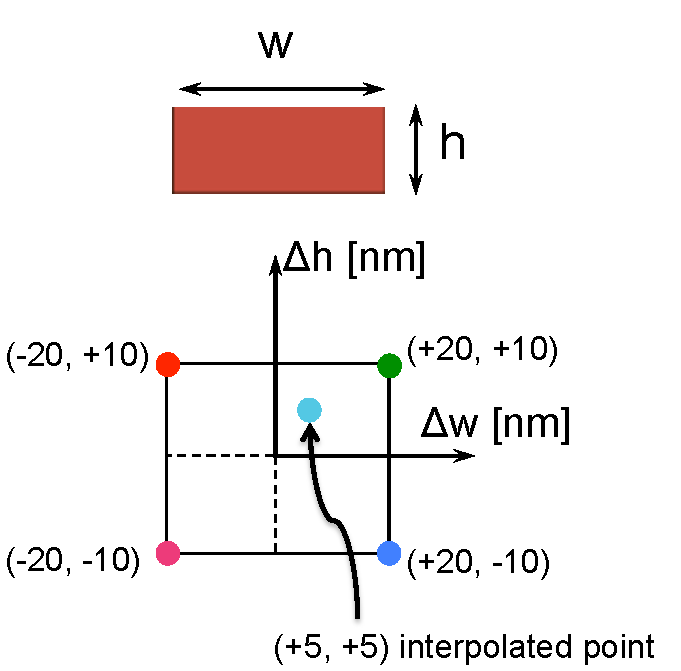
\includegraphics[width=0.35\linewidth]{../figs_chris/S_Interpolation1.pdf} } 
\subfloat[] {\label{S_Interpolation2}
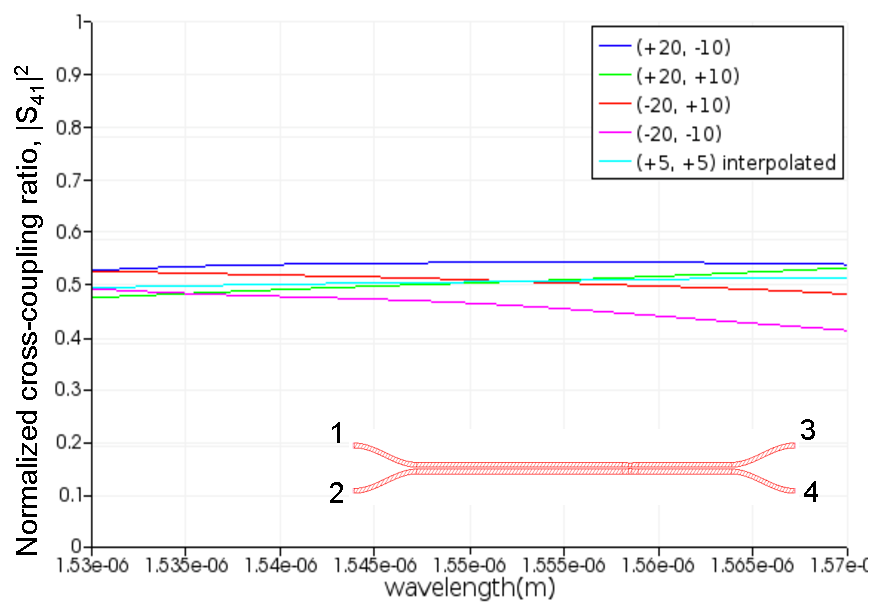
\includegraphics[width=0.5\linewidth]{../figs_chris/S_Interpolation2.pdf} } 
    \caption[]{(a) Process corners for two process parameters: waveguide height and width; (b) S-parameters for  a 2$\times$2  splitter, for the four process corners, and interpolated for an example geometry.}
    \label{s-interpolation}
\end{figure}

\begin{figure}[h]
	\centering
\subfloat[] {\label{MZI_simple_MC1}
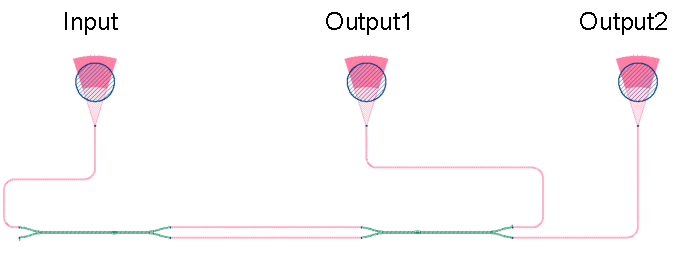
\includegraphics[width=0.5\linewidth]{../figs_chris/MZI_simple_MC1.pdf} } 
\subfloat[] {\label{MZI_simple_MC2}
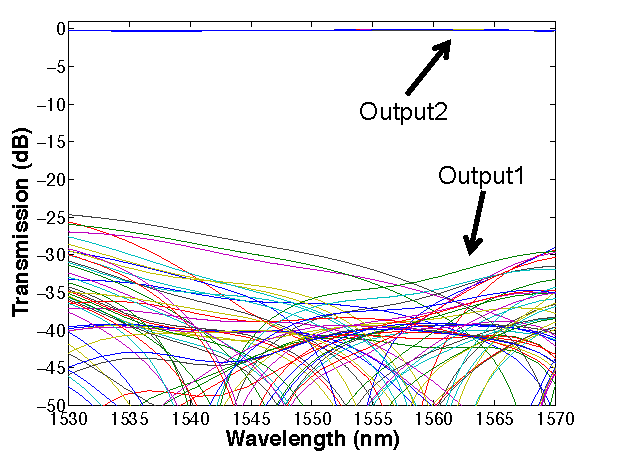
\includegraphics[width=0.5\linewidth]{../figs_chris/MZI_simple_MC2.pdf} } 
    \caption[]{(a) Layout of balanced Mach-Zehnder Interferometer test structure; (b) Monte Carlo simulation results for the output transmissions.}
    \label{MZI_common_MC}
\end{figure}

\subsubsection{Waveguides}
\label{sec:waveguide}
The waveguide transfer function of a waveguide is described by propagation properties such as loss, effective index, group index and dispersion, and need to be parameterized as a function of frequency, thickness and width. 
We can create parameterized models for the waveguide in a similar manner as in Section~\ref{SparamModel}, namely using interpolation.  We begin with 2D cross-section simulations of the waveguide (eigenmode simulations), and generate look-up tables for the effective index and group index for a range of geometries.  We then perform a multidimensional spline interpolation as above.

\subsubsection{Sub-circuit approach}
For the case of the Bragg grating, for example, we can assume that the manufacturing only affects the central Bragg wavelength.  If all other parameters remain the same (grating coupling coefficient) then a small perturbation to the nominal effective index can be applied.  This can be expressed as two independent linear parameters, $ \frac{\partial n_\text{eff}}{\partial w}$, and $ \frac{\partial n_\text{eff}}{\partial h}$, which are added to the nominal value.  Alternatively, we can use the waveguide model above as an input parameter to the Bragg grating compact model.  Specifically, the Bragg wavelength, $\lambda_B$, is determined by $\lambda_B = 2 n_\text{eff} \Lambda$, where $\Lambda$ is the grating period, and $n_\text{eff}$ is the effective index found in Section~\ref{sec:waveguide}.  In this latter approach, we can build up sub-circuits using a combination of primitive elements each with their own built-in manufacturing variability.

\subsection{Corner Analysis and a simple Monte Carlo}
\label{sec:corner}
In electronics design, it is common to perform a corner analysis on a circuit.  The designer chooses a model from an N-dimensional process variation parameter space, with $2^N$ choices.  Typically, N=2, as a result of two physical variations, and each variable is assigned whether the transistor is Slow (S), Typical (T) or Fast (F).  All transistors in the circuit use the same model, namely they all experience the same process variation.  This can be extended into a simple Monte Carlo analysis, where the transistor model is chosen to lie within the range of the process corners; this includes a distribution of process variables (e.g., truncated normal distribution). While this is useful in electronics in predicting the worst and best case for how fast a chip will operate (e.g., transimpedance amplifier for a detector, or a driver for a modulator), unfortunately this approach is not appropriate for photonics.  

First, we demonstrate this simple Monte Carlo approach on a small circuit, Figure~\ref{MZI_simple_MC1}, which is a Mach-Zehnder Interferometer consisting of two 2$\times$2 splitters connected with identical waveguides.  We assume that both devices and waveguides experience a common variability.  Here, the waveguide width and thickness are varied using a simple Monte Carlo simulation (where width and height are independent random variables), with the same values assigned to each component.  The results of the simulations are shown in  Figure~\ref{MZI_simple_MC2}, which show that the extinction ratio of the interferometer varies as a result of the simulated manufacturing variability.  The results obtained here are independent of the lengths and paths of the two waveguides, provided that the path length difference in the interferometer is $\Delta L = 0$ (i.e., a balanced interferometer). However, we know that from experiments, this is not the case.  

Experimental results for balanced interferometers (e.g., travelling wave modulators) show that a ``parasitic'' free-spectral (FSR) range is observed.  In some designs, this FSR can be quite easily observed in the optical spectrum, and corresponds to a large (several $\pi$) optical path difference.  The same is observed in identical ring resonators fabricated on the same die.  The within-die variations lead to a distribution of resonance frequencies.  Furthermore, experimental observations show that the variability between devices is correlated to distance between them.  For example, two ring resonators closely spaced will have similar resonance frequencies, while those drawn far apart will be highly mismatched.  This is common knowledge in analog circuit design, where critical paths are drawn closely together on the mask to minimize the differential error. 

In summary, corner analysis and simple Monte Carlo simulations where the variations are applied in common to the entire circuit are inappropriate for the study of circuit variability, since these do not include the spatial correlations that are experimentally observed.  They are, however, useful for predicting individual device variability (e.g., central wavelength of a Bragg grating or ring resonator).


\subsection{Monte Carlo with Spatial Correlations}

In electronics Monte Carlo simulations, it is possible to simulate circuits where a high degree of correlation exists between the variability of closely placed components.  This is included in the model using additional parameters (a mismatch parameter, or a correlation parameter).  The challenge for the designer is to determine these parameters based on a physical layout.
Ideally, Monte Carlo simulations should capture the die-to-die, device-to-device (intra-die), and intra-device variations, where the within-wafer variations have position-dependant correlations; models for correlation effects have been developed for electronic circuits \cite{agarwal2003statistical, liu2008spatial, cheng2011physically, zhang2013efficient, liao2015efficient}.  For example, for electronic circuit timing analysis, one approach is to group the devices using a partitioning quad-tree approach with each component being assigned several random variables depending on their location in the circuit  \cite{agarwal2003statistical}.  

In photonics, correlated yield analysis is attracting increasing attention, and there have been several studies investigating the statistical on-chip correlations \cite{lukas14:OFC,hochberg:wafer}, and models for dealing with the uncertainty of devices \cite{MIT:uncertainty}.  From this past work, what is clear is that if only common-mode variability is considered (corner analysis or simple Monte Carlo, described in Section~\ref{sec:corner} above), the simulations do not capture an important type of variability -- differential, or spatially correlated variability.  Namely, two nominally identical devices side-by-side on a chip will have slightly difference performance.  This difference can have significant impact on system performance (e.g., WDM ring resonators, optical switches) and it cannot be simply compensated by thermally tuning the entire chip, but rather requires individual tuning for each component.  Clearly tuning every single component in a silicon photonics circuit is prohibitive, hence we require a tool to determine which components need to be tuned.  This can be determined by a Monte Carlo analysis that takes spatial correlations into account.

In this work, we propose a methodology that takes correlation between devices into account by using the physical layout in order to perform a manufacturing variability analysis of on-chip photonic integrated circuits.  We create a virtual wafer in each Monte Carlo iteration, and each device determines its parameter within the wafer map on the basis of the physical mask layout.
Our methodology  provides insight into the significance of compact layouts for photonic designs, and offers a useful tool for post-layout verification and power trimming estimation.

\begin{figure}[h]
    \centering
\subfloat[] {\label{flow_chart}
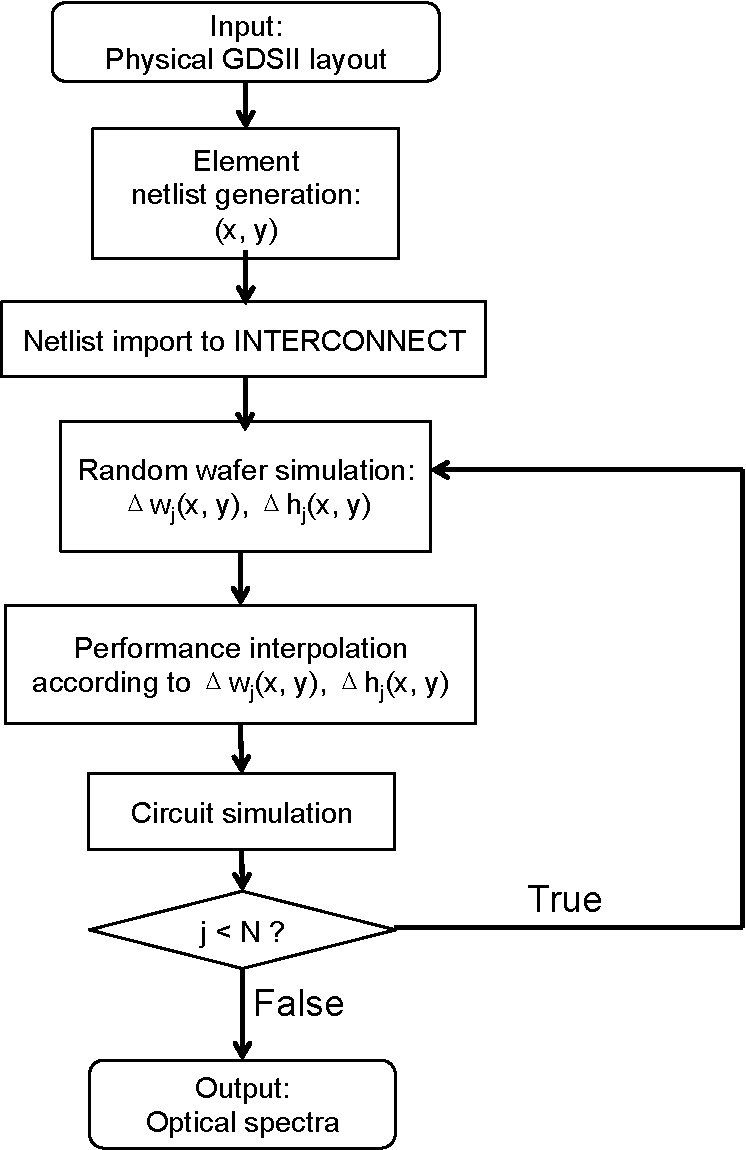
\includegraphics[width=0.35\linewidth]{../figs_chris/flow_chart.pdf} } 
\subfloat[] {\label{wafer_maps}
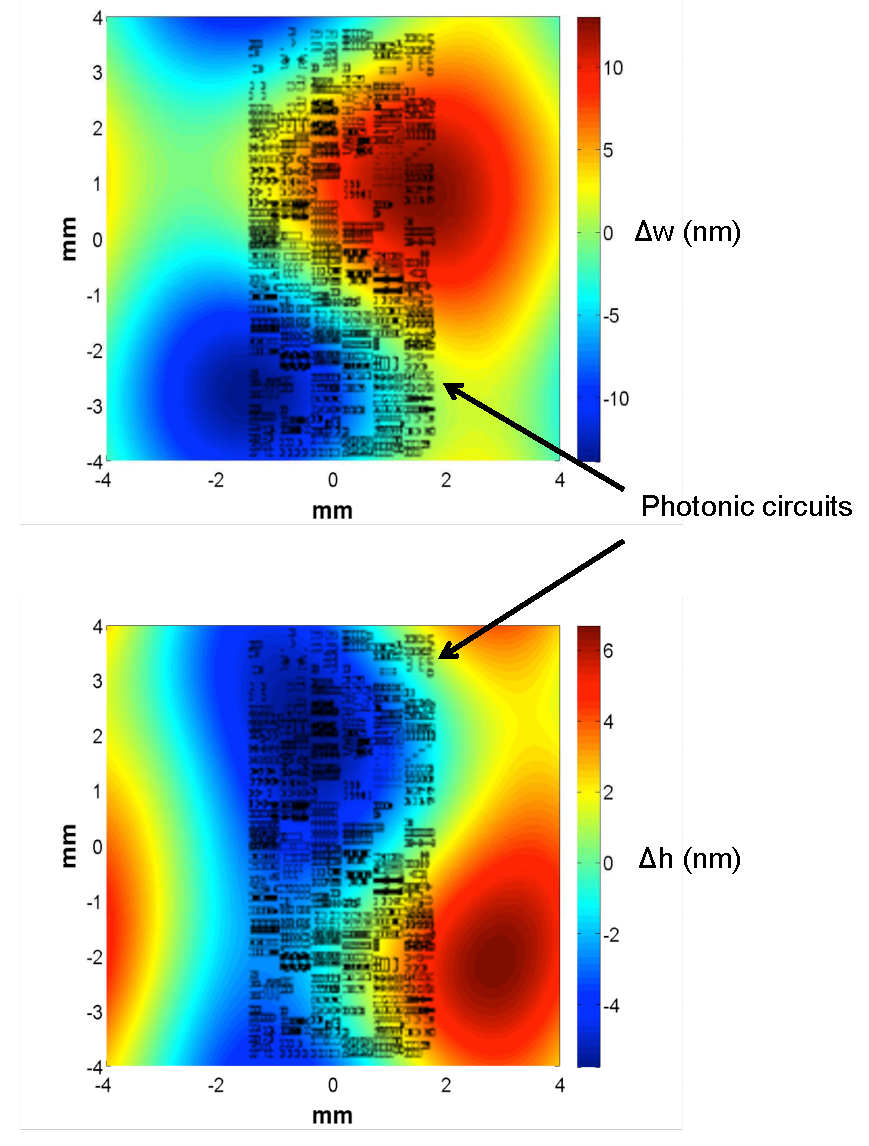
\includegraphics[width=0.4\linewidth]{../figs_chris/wafer_maps.pdf} } 
    \caption{(a) Flow chart of the proposed methodology; (b) simulated waveguide linewidth ($\Delta w$) and thickness ($\Delta h$) deviations across a wafer.} 
\end{figure}

Figure \ref{flow_chart} shows the flow chart of our proposed methodology. The procedure includes: 
\begin{itemize}
\item First, the layout for silicon photonic circuits and/or devices under test are created.  In the example presented here, they are designed using KLayout \cite{www_klayout}. 
\item
The netlist is extracted from the layout, either using Mentor Graphics LVS or the SiEPIC-EBeam-PDK add-on \cite{siepic-ebeam-pdk} to KLayout \cite{www_klayout}.  The netlist provides a list of the primitive components in the library and the connectivity between components.  The netlist is imported into Lumerical INTERCONNECT for circuit simulations. 
\item
The third step is the generation of a virtual wafer.  Silicon waveguide width deviations, $\Delta w(x,y)$, and wafer thickness deviations, $\Delta h(x,y)$, are simulated across the chip, as illustrated in the maps in Figure~\ref{wafer_maps}. Both deviations are characterized by a sigma RMS amplitude and a correlation length, and both are based on experimental results \cite{lukas14:OFC,hochberg:wafer}. In each run of the Monte Carlo simulation, different deviation maps are be generated in Lumerical INTERCONNECT.
\item
According to the spatially-dependent waveguide width and thickness map, the optical S-parameters of primitive elements and the optical propagation constants of connecting waveguides are calculated.  This is performed using interpolation in INTERCONNECT as described in Section~\ref{SparamModel}. 
\item
The circuit with components updated based on their positions is simulated.  This is repeated several times, and the results can be visualized, as in Figure~\ref{MZI_circuit2_MC}. 
\end{itemize}

\begin{figure}[t]
    \centering
\subfloat[] {\label{MZI_spatial_MC1}
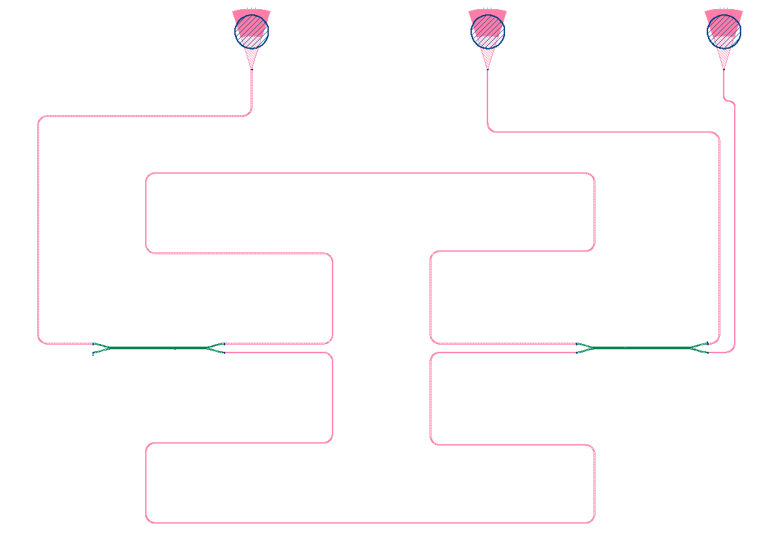
\includegraphics[width=0.5\linewidth]{../figs_chris/MZI_spatial_MC1.pdf} } 
\subfloat[] {\label{MZI_spatial_MC2}
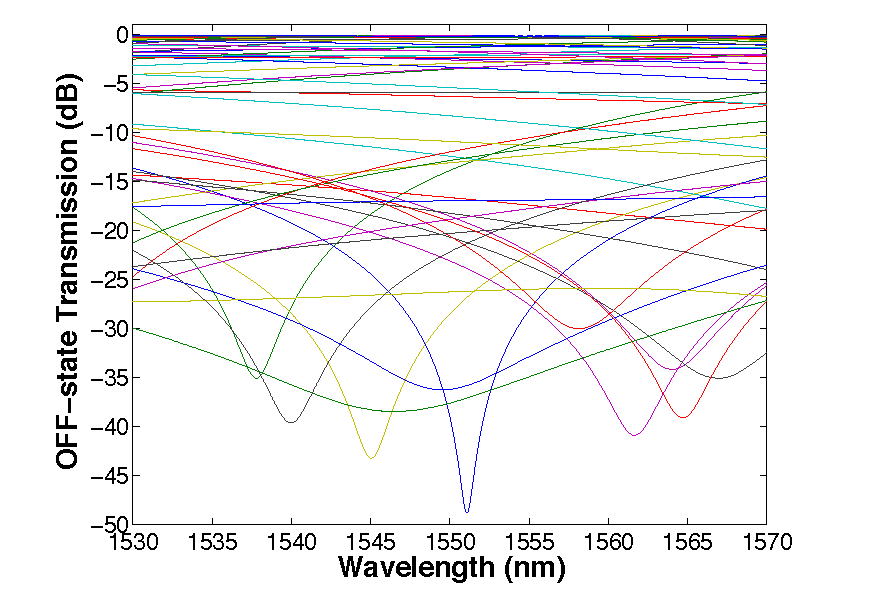
\includegraphics[width=0.5\linewidth]{../figs_chris/MZI_spatial_MC2.pdf} } 
    \caption{(a) Layout of balanced Mach-Zehnder Interferometer test structure; (b) Monte Carlo simulation results for the output transmissions.} 
    \label{spatial}
\end{figure}


%The scatter plot in Figure~\ref{error} shows the simulated phase error of a balanced Mach-Zehnder Interferometer versus the waveguide spacing between two arms, in a 248 nm silicon photonics process. In the Monte Carlo simulations, the horizontal length of the phase arms, $L$,  is 200 $\mu m$. The phase error is defined as the absolute optical phase difference between the two phase arms. Ideally, the phase error should be 0 when there are no fabrication variations. However, this figure clearly shows that the mean of the phase error for an ensemble of MZIs is approximately linearly proportional to the waveguide spacing, emphasizing the importance of very compact layout designs, particularly where phase matching is required.  This simulation is similar to the proportionality  observed experimentally in ring resonators \cite{lukas14:OFC}.  The simulated phase error can be used to estimate the trimming power required for MZI-based photonic switches. 
Now, we demonstrate this approach on a large Mach-Zehnder interferometer consisting of two 2$\times$2 splitters connected with identical waveguides, as shown in Figure~\ref{MZI_spatial_MC1}. Compared with the test structure in Figure~\ref{MZI_simple_MC1}, here the phase arms of the MZI are much longer and are further apart in space.  The results of the simulations are shown in Figure~\ref{MZI_spatial_MC2}, which show that the extinction ratio of the interferometer is no longer distinguishable due to the spatially dependent phase errors.

Another example application of the Monte Carlo method is for the Dual Phase Shifted Waveguide Bragg Grating (DPS-WBG) \cite{burla2013integrated, bedard2016dual}.  
This device has applications for microwave photonics (true time delay, TTD, for broadband microwave signals) \cite{burla2013integrated} and high-speed data communication (Bragg grating modulator) \cite{bedard2016dual}.  
It consists of a coupled cavity, similar to coupled ring resonators, except that it is implemented using three Bragg gratings with a quarter-wavelength phase shift section separating each grating, as shown in Figure~\ref{DPSWBG_gds}.  
In the ideal case, the resonance frequency of the two cavities is perfectly matched.  
However, differential manufacturing errors lead to the gratings being slightly different, which results in the splitting of the two modes.  
The central peak in the transmission of the device is highly sensitive to this variation; namely the peak's insertion loss varies.  
What is more remarkable is the reflection spectrum. In the ideal case, there is a dip at the resonance frequency.  
With a slight mismatch between the components, the peak can completely vanish; this device now operates as an all-pass filter with a phase shift.  
The transmission and reflection spectrum can also be tuned by heating each section.  
What is important to note for this sub-circuit / compound device is that manufacturing variability needs to be taken into account in order to have a correct understanding of  its performance.


\begin{figure}[tbp]
\begin{center}   
\subfloat[Illustration of a Dual Phase Shifted Waveguide Bragg Grating (DPS-WBG).  Note that the simulated device had 100 grating periods in the left and right sections, and 200 grating periods in the middle section.]{\label{DPSWBG_gds} 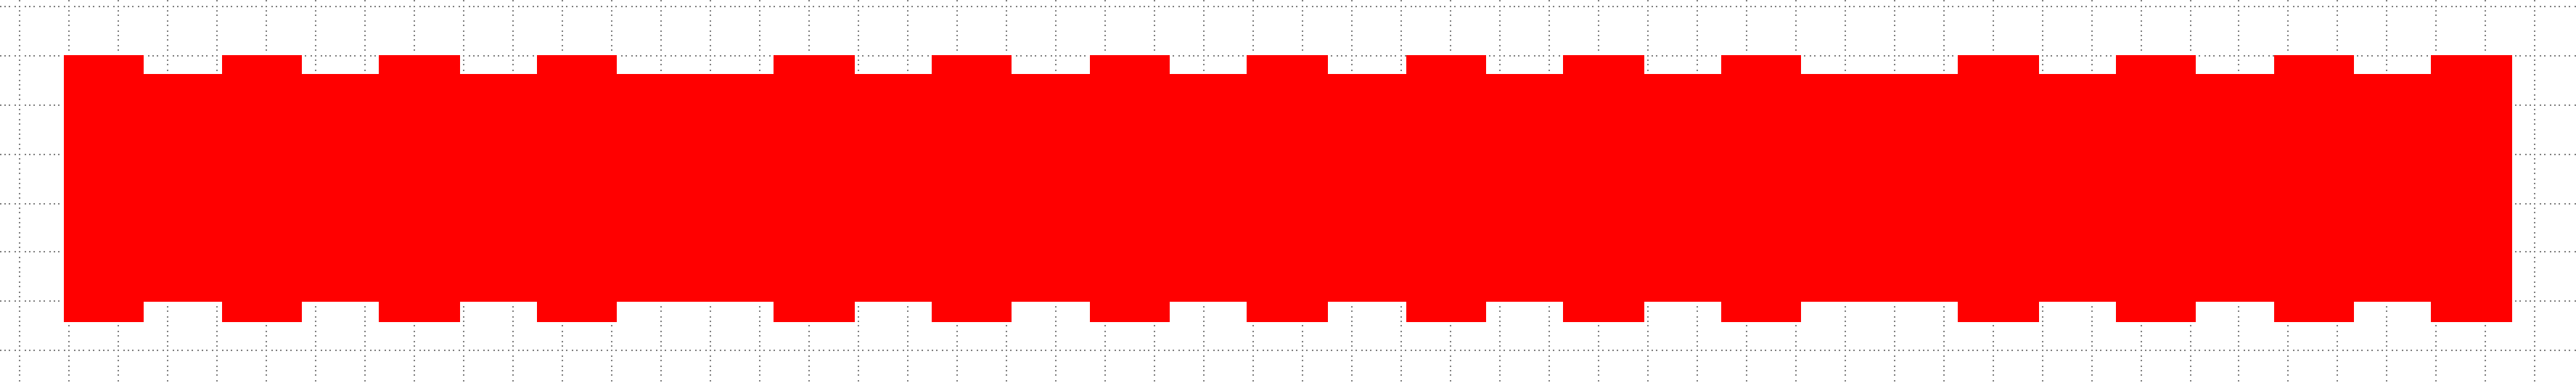
\includegraphics[width=0.7\linewidth]{../figs_paper/DPSWBG_gds2} } \\
%\subfloat[Layout of a Dual Phase Shifted Waveguide Bragg Grating (DPS-WBG).]{\label{DPSWBG_gds} 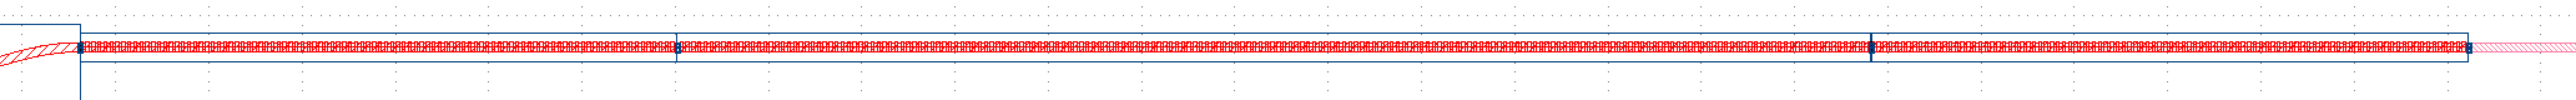
\includegraphics[width=\linewidth]{../figs_paper/DPSWBG_gds} } \\
\subfloat[Circuit simulation of the nominal design] {\label{DPSWBG1}
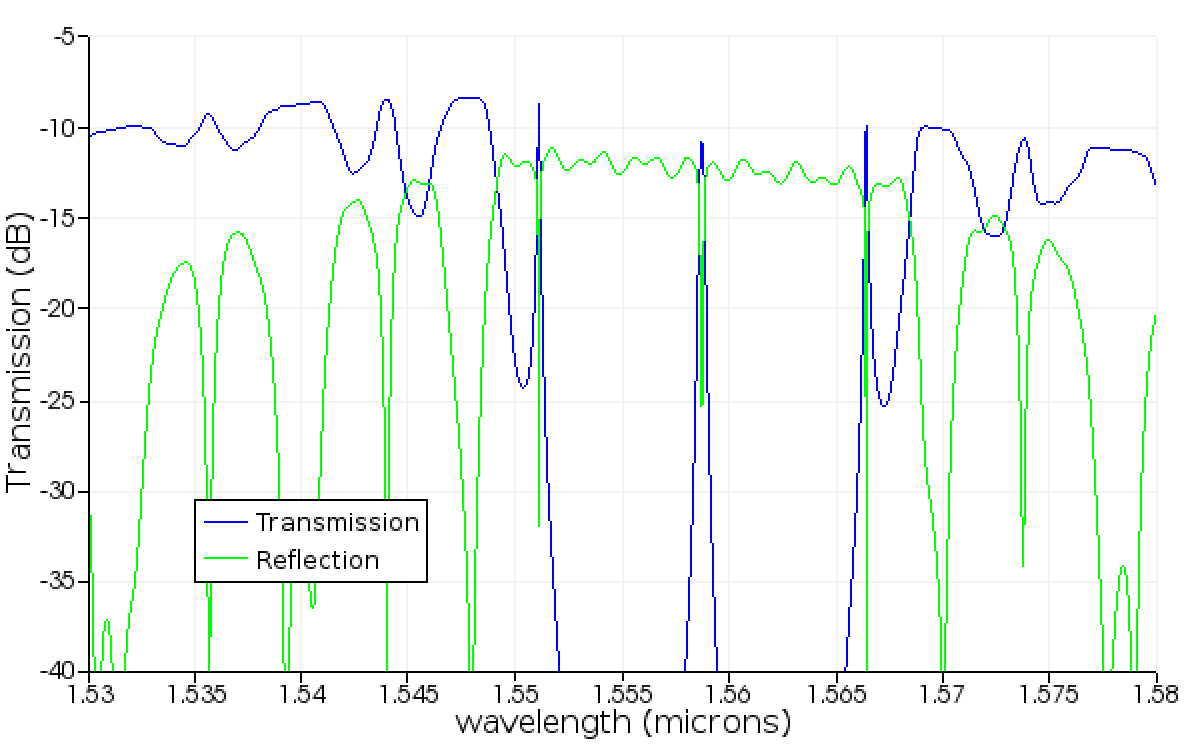
\includegraphics[width=0.4\linewidth]{../figs_paper/DPSWBG1} }
\subfloat[Monte Carlo circuit simulation including spatial correlations (one simulation).] {\label{DPSWBG2}
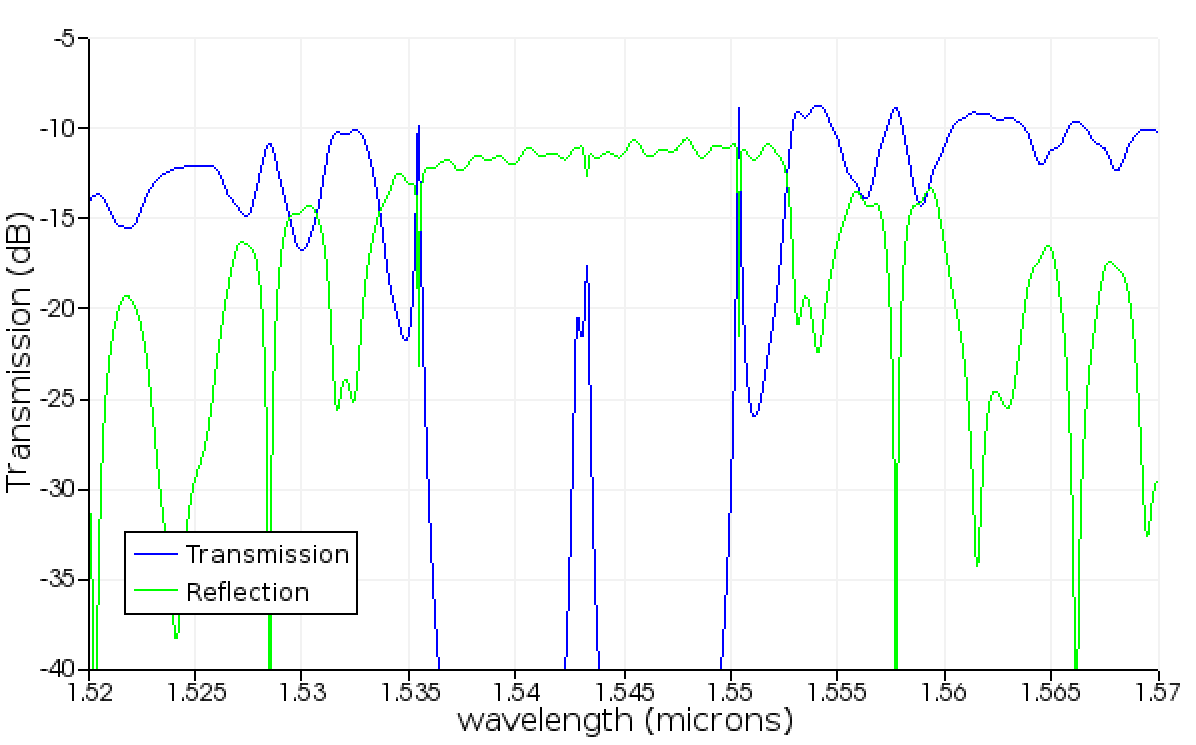
\includegraphics[width=0.4\linewidth]{../figs_paper/DPSWBG2} }
\caption{Layout and simulations of a Dual Phase Shifted Waveguide Bragg Grating (DPS-WBG) \cite{burla2013integrated}.}
\label{Bragg}
\end{center}
\end{figure}


\section{Conclusion}\label{sec6}

In this paper, we described a design methodology that takes advantage of CMOS Electronic Design Automation (EDA) tools coupled to optical design software.  Whether the design is implemented using a schematic-first or a layout-first approach, incorporating manufacturing yield and process variations into the design flow is a critical step in the functional verification of the circuit.  Simulating process variation impact on photonic circuits is performed by 1) synchronizing the schematic with the as-drawn layout using a netlist extraction approach that includes component position data, and 2) using a Monte Carlo analysis that includes layout-specific spatial correlation effects made possible by creating virtual wafer maps and using parameterized optical component models.
The  objective of the design flow is ``first-time-right'' design, where circuits function correctly the first time they are fabricated; this can be achieved only if the designer takes manufacturing challenges into consideration and applies effective mitigation strategies in order to build circuits that are immune to these variations.

%Full-flow design environments are becoming a reality for silicon photonics.
%
%The mature CMOS fabrication processes and multi-project wafer (MPW) fabrication runs 
%%Stable processes that are repeatable
%enable the development of component libraries for system design.  
%
%Similar to the electronics industry, photonic integrated circuit design and fabrication is evolving towards specialized roles, namely: a) fabrication and processing, b) EDA tools; c) component, library, and PDKs; and, d) system design.  This separation of roles will lead to accelerated product development and ultimately aiding the silicon photonics industry achieve its objectives. 




\acknowledgments

The authors would like to thank CMC Microsystems for enabling the fabrication of numerous chips via imec-ePIXfab and IME.  Funding for this research was provided by NSERC, particularly the NSERC CREATE Silicon Electronic Photonic Integrated Circuits (SiEPIC) training program, \url{http://www.siepic.ubc.ca}, and Huawei Canada.

\bibliography{../Refs/references}
\bibliographystyle{spiebib33}


\end{document}
